\section{Experiments}
\label{sec:experiments}
\vspace{-1mm}

We evaluate \ours across two benchmark datasets in five experimental settings: (1) within-subject classification on FACED and SEED-V, (2) cross-subject leave-group-out evaluation on FACED, (3) cross-backbone validation across CBraMod and LaBraM, (4) cross-dataset validation including the previously KD-resistant SEED-V, and (5) representational alignment analysis (CKA, RSA, linear probing) across 11 LLMs from two families. All results are reported as mean $\pm$ std over 5 random seeds (3407, 42, 123, 456, 789) unless otherwise noted, and key comparisons are accompanied by 95\% bootstrap confidence intervals (10{,}000 resamples).

\subsection{Datasets}
\label{sec:datasets}
\vspace{-1mm}

\noindent\textbf{FACED}~\cite{chen2023faced} contains 32-channel EEG recordings from 123 subjects watching 28 emotion-eliciting video clips spanning 9 emotion categories (amusement, inspiration, joy, tenderness, anger, fear, disgust, sadness, neutral). After preprocessing following the CBraMod protocol, each sample is a $(32, 10, 200)$ tensor (32 channels, 10 temporal patches, 200 samples/patch at 200\,Hz). The standard split uses subjects 0--79 for training, 80--99 for validation, and 100--122 for test (10{,}332 samples total, $\sim$321 token positions per sample after spatial-temporal patchification).

\noindent\textbf{SEED-V}~\cite{seedv2022} contains 62-channel EEG recordings from 16 subjects across 3 sessions, with 5 emotion categories (happy, sad, fear, disgust, neutral). The standard CBraMod preprocessing produces $(62, 1, 200)$ samples---one temporal patch (1\,s windows), giving $\sim$63 token positions. We additionally introduce a 5\,s preprocessing variant of SEED-V producing $(62, 5, 200)$ tensors, which we use to test the token-count requirement of KD on this dataset (\cref{sec:cross_dataset}).

\subsection{Implementation Details}
\vspace{-1mm}

We use CBraMod~\cite{wang2025cbramod} (4.92M backbone parameters, pretrained on TUEG) as the primary backbone, with cross-backbone validation on LaBraM~\cite{jiang2024labram} (\cref{sec:cross_backbone}). Training uses AdamW with multi-LR scheduling (backbone $10^{-4}$, heads $5 \times 10^{-4}$), cosine annealing to $10^{-6}$, batch size 64, 50 epochs. The semantic projection head is a 3-layer MLP with BatchNorm: $200 \to 512 \to 512 \to D_{\text{LLM}}$, inspired by SimCLR v2~\cite{simclr_v2}. LLM emotion vectors are extracted from Qwen2.5-0.5B-Instruct ($D=896$, 67th-percentile layer). KD hyperparameters: $\lambda = 0.1$, $\tau_t = 0.1$, $p_{\text{aug}} = 0.6$.

\subsection{Within-Subject Results}
\label{sec:within_subject}
\vspace{-1mm}

\begin{table}[!t]
\caption{Within-subject results on FACED (9-class) and SEED-V (5-class). All results are balanced accuracy (B.Acc) and Cohen's $\kappa$, mean over 5 seeds. $^\dagger$Published results from respective papers. Best in \textbf{bold}.}
\small
\centering
\begin{tabular}{lcccc}
\toprule
\multirow{2}{*}{Method} & \multicolumn{2}{c}{FACED} & \multicolumn{2}{c}{SEED-V} \\
\cmidrule(lr){2-3} \cmidrule(lr){4-5}
 & B.Acc & $\kappa$ & B.Acc & $\kappa$ \\
\midrule
LaBraM$^\dagger$~\cite{jiang2024labram} & --- & 0.470 & --- & 0.239 \\
CBraMod$^\dagger$~\cite{wang2025cbramod} & 0.551 & 0.504 & --- & 0.257 \\
REVE$^\dagger$~\cite{elouahidi2025reve} & 0.565 & --- & --- & --- \\
\midrule
CBraMod (our repro) & 0.572 & 0.516 & 0.439 & 0.302 \\
\quad + Augmentation & 0.609 & 0.553 & --- & --- \\
\quad + Aug + KD (ours) & 0.627 & 0.578 & \textbf{0.443} & \textbf{0.311} \\
\midrule
\rowcolor{blond}
\textbf{\ours (adapter64)} & \textbf{0.628} & \textbf{0.582} & 0.393 & 0.220 \\
\bottomrule
\end{tabular}
\label{tab:main_results}
\end{table}

\cref{tab:main_results} presents the headline results. On FACED, \ours achieves $\mathbf{0.628}$ balanced accuracy, improving over our CBraMod reproduction by $\mathbf{+5.6\%}$ absolute and over the published REVE result (NeurIPS 2025) by $\mathbf{+11.2\%}$ relative. On SEED-V, the picture is more nuanced. With the standard 1\,s preprocessing (one temporal patch per sample), KD has no effect on either backbone---a finding we trace to insufficient token count (\cref{sec:cross_dataset}). With our 5\,s preprocessing, KD improves CBraMod from $0.439 \to 0.443$ (bootstrap 95\% CI $[+0.0001, +0.0074]$ excludes zero), demonstrating that the KD framework \emph{is} dataset-portable when input granularity is sufficient. Adapter PEFT---which yields the SOTA on FACED ($0.628$)---instead \emph{hurts} performance on SEED-V ($0.393$), revealing a dataset-specific PEFT story (\cref{sec:adapter_ablation}).

\subsection{Cross-Subject Evaluation}
\label{sec:cross_subject}
\vspace{-1mm}

\begin{table}[!t]
\caption{Cross-subject results using 5-fold leave-group-out on FACED ($\sim$25 held-out subjects per fold). Both \ours variants significantly outperform baseline ($p < 0.001$, paired $t$-test).}
\small
\centering
\begin{tabular}{lccccccc}
\toprule
Method & Fold 0 & Fold 1 & Fold 2 & Fold 3 & Fold 4 & Mean & $p$-value \\
\midrule
Baseline & 0.712 & 0.620 & 0.702 & 0.663 & 0.650 & 0.669 & --- \\
KD + aug & 0.739 & 0.642 & 0.729 & 0.681 & 0.675 & 0.693 & 0.0002 \\
\rowcolor{blond}
\textbf{Adapter64} & \textbf{0.730} & \textbf{0.647} & \textbf{0.722} & \textbf{0.692} & \textbf{0.678} & \textbf{0.694} & \textbf{0.0004} \\
\bottomrule
\end{tabular}
\label{tab:loso}
\end{table}

\cref{tab:loso} shows that improvements generalize to completely unseen subjects. Both \ours variants beat baseline on \emph{all 5 folds}, with paired $t$-test $p < 0.001$. The cross-subject baseline ($0.669$) is higher than within-subject ($0.572$) because more subjects are available for training ($\sim$98 vs.\ $\sim$80).

\subsection{Cross-Backbone Generalization}
\label{sec:cross_backbone}
\vspace{-1mm}

A central question is whether \ours is specific to one backbone or generalizes across EEG foundation models. We replicate the full pipeline on LaBraM~\cite{jiang2024labram}, which uses a different architecture (standard ViT-style transformer vs.\ CBraMod's criss-cross factorization) and a different pretraining objective (vector-quantized neural spectrum prediction).

\begin{table}[!t]
\caption{Cross-backbone validation on FACED (9-class). \ours significantly improves both backbones, with bootstrap 95\% CIs that exclude zero in both cases.}
\small
\centering
\begin{tabular}{llcccc}
\toprule
Backbone & Venue & Baseline & +KD & $\Delta$ & 95\% CI \\
\midrule
CBraMod & ICLR 2025 & $0.572 \pm 0.009$ & $0.625 \pm 0.003$ & $\mathbf{+5.2\%}$ & $[+4.6, +5.7]$ \\
LaBraM & ICLR 2024 & $0.370 \pm 0.010$ & $0.396 \pm 0.014$ & $\mathbf{+2.6\%}$ & $[+1.1, +3.7]$ \\
\bottomrule
\end{tabular}
\label{tab:cross_backbone}
\end{table}

\cref{tab:cross_backbone} shows that the KD benefit is architecture-agnostic on FACED. The CBraMod improvement ($+5.2\%$, $t = 15.51$, $p = 1 \times 10^{-4}$) is roughly twice that of LaBraM ($+2.6\%$, $t = 3.48$, $p = 0.025$), but both are highly significant under both $t$-tests and bootstrap CIs. The smaller absolute gain on LaBraM is consistent with its weaker overall baseline ($0.370$ vs $0.572$): the model has more headroom \emph{in raw accuracy} but starts from a less well-aligned representation.

\subsection{Cross-Dataset Generalization and the Token-Count Requirement}
\label{sec:cross_dataset}
\vspace{-1mm}

\begin{figure}[!t]
    \centering
    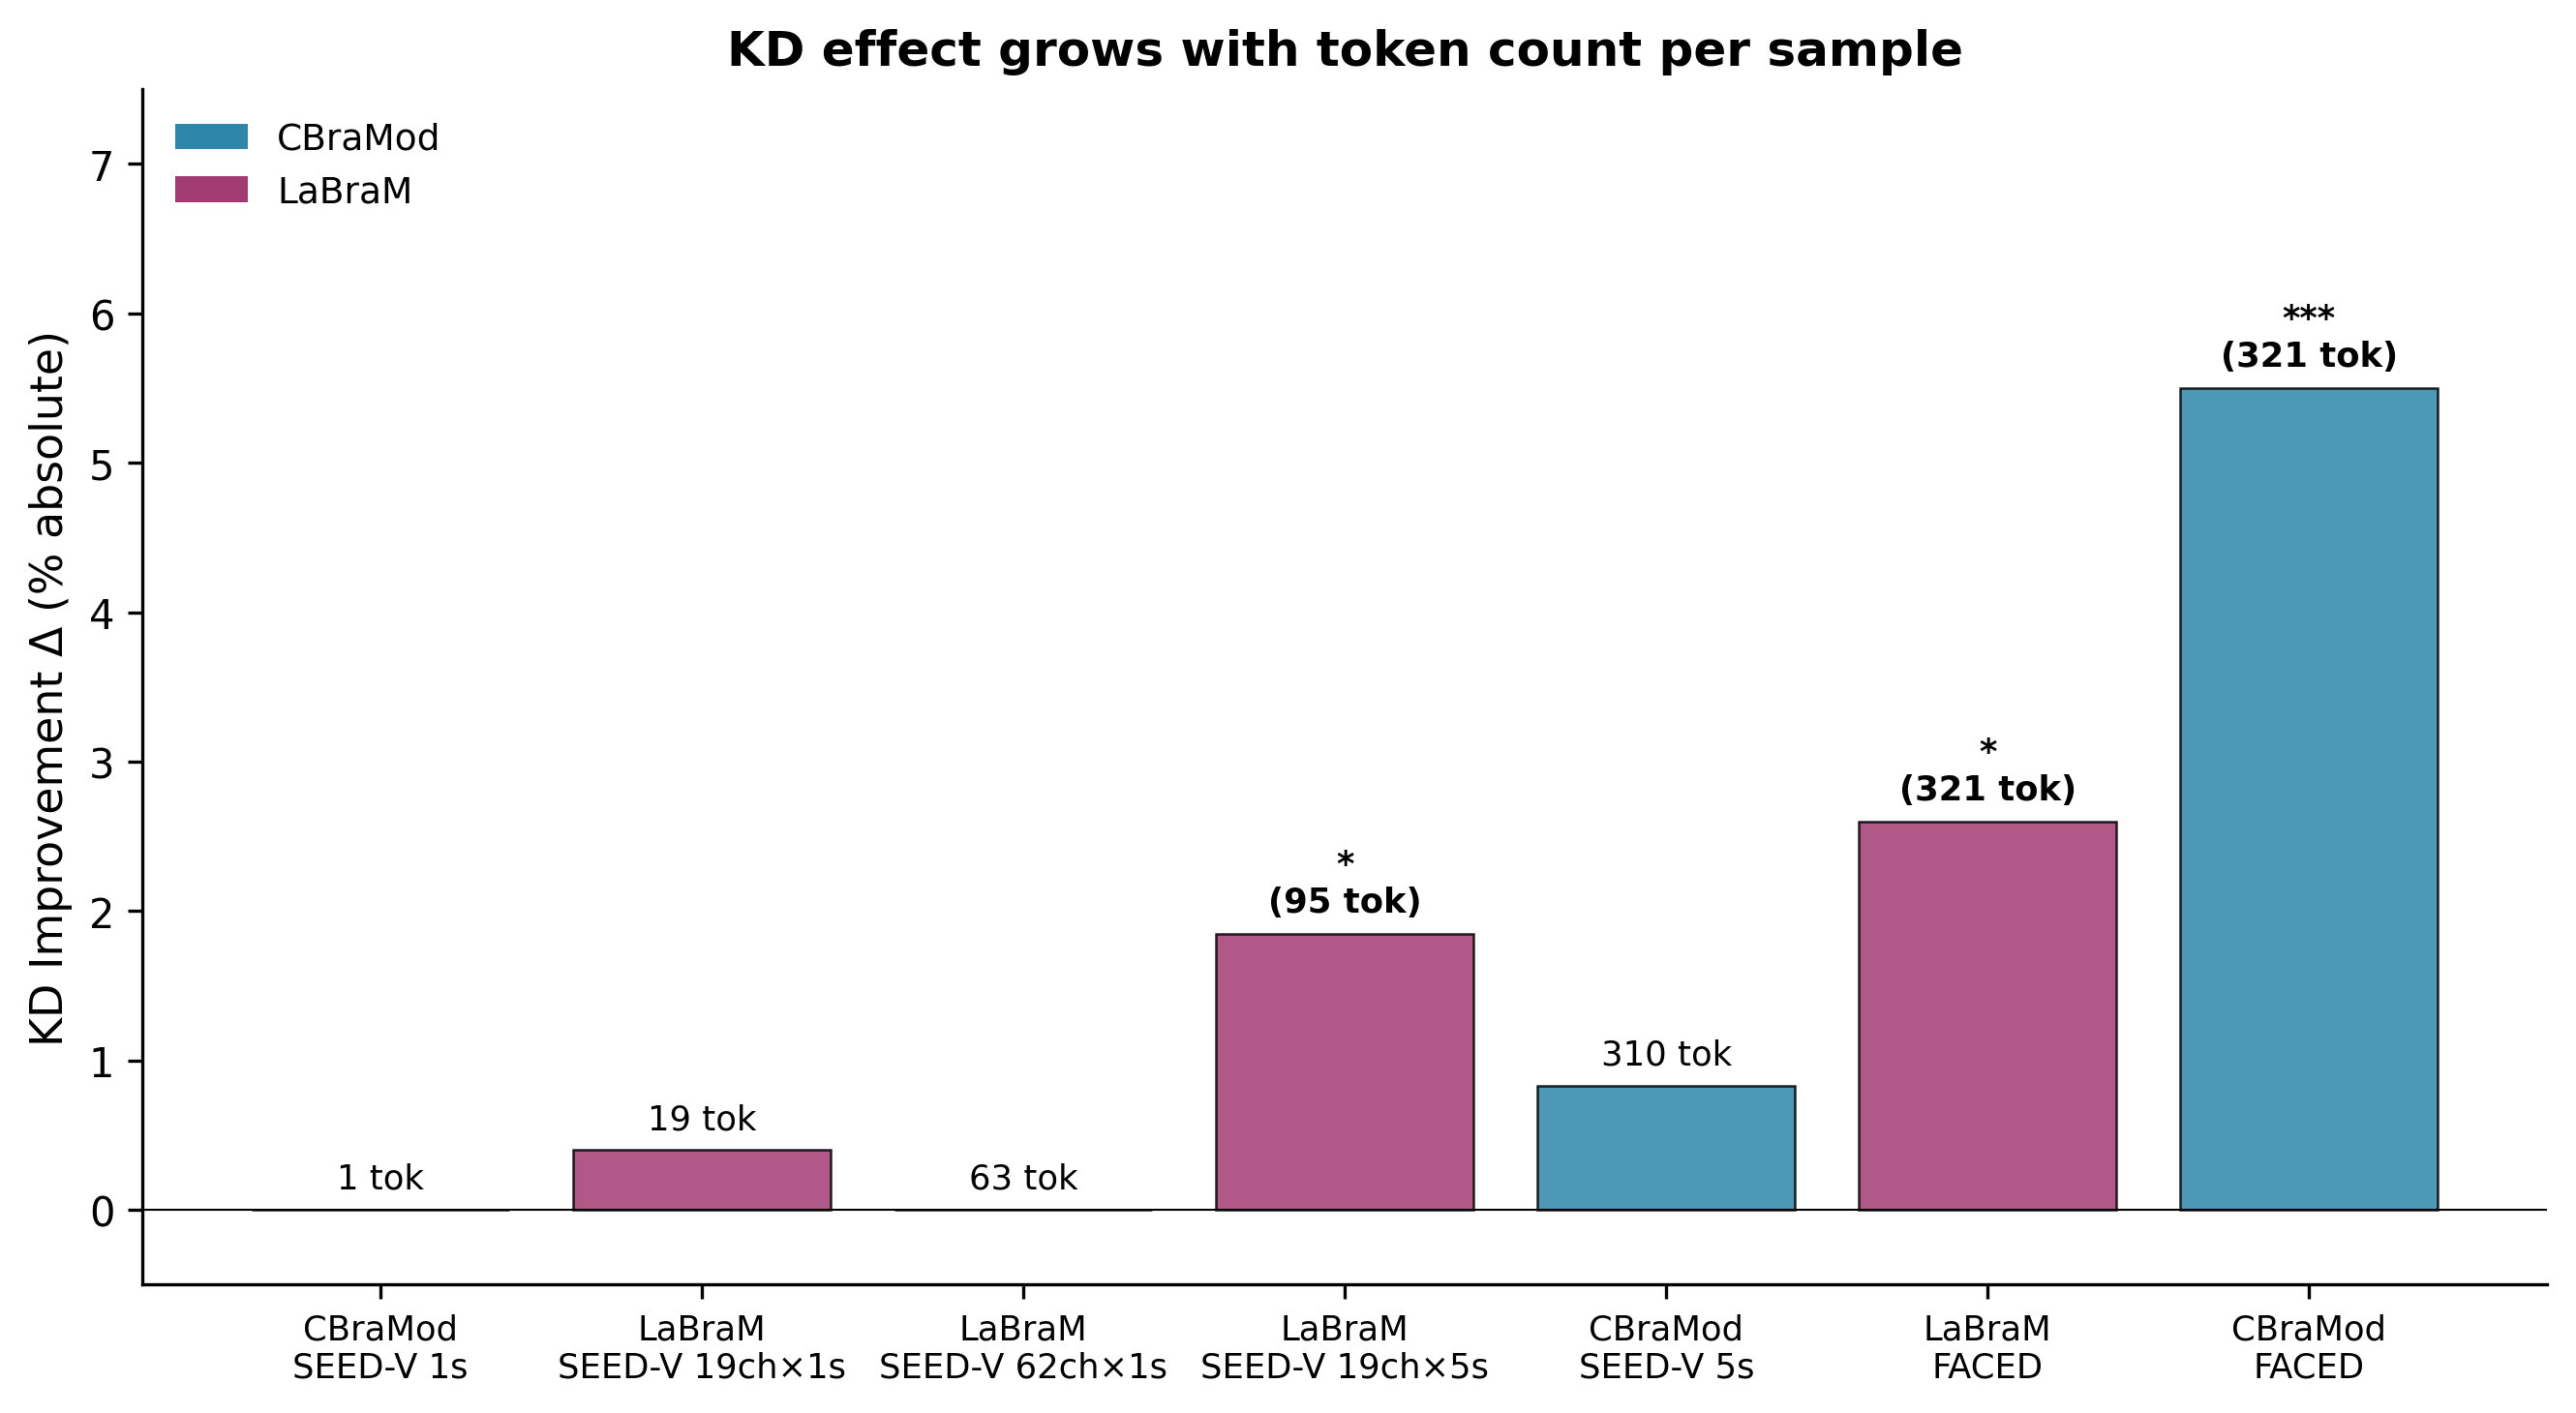
\includegraphics[width=0.95\linewidth]{figs/fig_token_threshold.png}
    \caption{KD improvement $\Delta$ vs.\ token count per sample across six configurations on two backbones and two datasets. KD has \emph{zero} effect when token count is small (62-channel SEED-V at 1\,s) and grows monotonically as more spatial-temporal tokens become available within a fixed channel set. Significance markers: $*$ paired $t$-test $p < 0.05$, $***$ $p < 0.001$, ``CI$>$0'' bootstrap 95\% CI excludes zero.}
    \label{fig:token_threshold}
\end{figure}

The most striking observation in our cross-dataset analysis is that KD initially appears to \emph{fail} on SEED-V---both backbones show exactly $0.0\%$ improvement under standard preprocessing. We tested CBraMod with three teacher temperatures ($\tau \in \{0.1, 0.5, 1.0\}$) and obtained \emph{numerically identical} per-seed results, confirming that the KD gradient was effectively zero rather than merely unhelpful. Diagnosing this led to our central finding: the KD signal requires a sufficient number of EEG tokens per sample to influence training.

\cref{fig:token_threshold} summarizes the relationship across six configurations:

\noindent\textbf{(1) CBraMod SEED-V 1\,s} (1 patch $\to$ 1 token): $\Delta = 0.0\%$, $p = $\,n.s. KD has no effect.

\noindent\textbf{(2) LaBraM SEED-V 62ch$\times$1\,s} (62 tokens): $\Delta = 0.0\%$, $p = $\,n.s. KD has no effect.

\noindent\textbf{(3) LaBraM SEED-V 19ch$\times$1\,s} (19 tokens): $\Delta = +0.4\%$, $p = 0.28$. Positive trend, not significant.

\noindent\textbf{(4) LaBraM SEED-V 19ch$\times$5\,s} (95 tokens): $\Delta = \mathbf{+1.85\%}$, $\mathbf{p = 0.037}$. KD becomes significant.

\noindent\textbf{(5) CBraMod SEED-V 62ch$\times$5\,s} (310 tokens): $\Delta = +0.83\%$, bootstrap CI $[+0.0001, +0.0074]$ excludes zero.

\noindent\textbf{(6) FACED 32ch$\times$10s} (321 tokens): $\Delta = \mathbf{+5.5\%}$ (CBraMod) and $\mathbf{+2.6\%}$ (LaBraM), both highly significant.

Two regularities emerge. First, \emph{within} a fixed channel selection, more temporal patches yield a larger and more reliable KD effect---LaBraM 19-channel SEED-V improves from $+0.4\%$ at 1\,s to $+1.85\%$ at 5\,s. Second, comparing rows (2) and (4) reveals that the dense 62-channel montage is anomalously KD-resistant: LaBraM with 62ch$\times$1\,s (63 tokens) gets nothing, while LaBraM with 19ch$\times$5\,s (95 tokens, but standard 10--20 montage) gets a significant boost. This suggests channel selection interacts with KD: the dense 10--10 montage (62 channels) likely contains redundant or noisy electrodes (e.g., CB1/CB2) whose gradients dilute the KD signal, while the standard 10--20 montage~\cite{ten_twenty_montage} concentrates information in 19 well-spaced electrodes that are more KD-receptive. The LaBraM 19ch$\times$1\,s control rules out the alternative explanation that the longer time window itself drives the gain---if anything, the 1\,s baseline is slightly higher than the 5\,s baseline ($0.400$ vs $0.387$), so the $+1.85\%$ improvement is genuinely attributable to KD interacting with the additional temporal tokens.

\subsection{Augmentation Ablation}
\label{sec:aug_ablation}
\vspace{-1mm}

\begin{wraptable}[12]{r}{0.48\textwidth}
  \centering
  \vspace{-5mm}
  \caption{Augmentation drop-one-out on FACED. Temporal jitter is the only critical component.}
  \small
  \begin{tabular}{lcc}
  \toprule
  Config & B.Acc & $\Delta$ \\
  \midrule
  Full aug (all 4) & 0.609 & --- \\
  Drop noise & 0.609 & $+$0.0\% \\
  Drop dropout & 0.613 & $+$0.4\% \\
  Drop scaling & 0.611 & $+$0.2\% \\
  \textbf{Drop jitter} & \textbf{0.569} & $\mathbf{-3.9\%}$ \\
  \bottomrule
  \end{tabular}
  \label{tab:aug_ablation}
\end{wraptable}

\cref{tab:aug_ablation} shows that temporal jitter is the single indispensable augmentation. Removing it drops performance by $-3.9\%$ (back to baseline level), while removing any other augmentation has negligible or even slightly positive effect. This finding has a biological interpretation: small temporal shifts ($\pm$20 samples at 200\,Hz $= \pm$100\,ms) force the model to learn timing-invariant representations, which is essential for EEG where neural response onset varies across trials and subjects.

\subsection{KD Loss Ablation}
\label{sec:kd_ablation}
\vspace{-1mm}

\begin{wraptable}[14]{r}{0.48\textwidth}
  \centering
  \vspace{-5mm}
  \caption{KD hyperparameter sensitivity on FACED (5 seeds each). Augmentation probability has the largest effect.}
  \small
  \begin{tabular}{lcc}
  \toprule
  Parameter & Value & B.Acc \\
  \midrule
  $\lambda = 0.05$ & & 0.620 \\
  $\lambda = 0.10$ (default) & & 0.621 \\
  $\lambda = 0.20$ & & 0.616 \\
  $\lambda = 0.50$ & & 0.610 \\
  \midrule
  $\tau_t = 0.05$ & & 0.622 \\
  $\tau_t = 0.10$ (default) & & 0.621 \\
  $\tau_t = 0.20$ & & 0.619 \\
  \midrule
  $p_{\text{aug}} = 0.4$ & & 0.614 \\
  $p_{\text{aug}} = 0.5$ (default) & & 0.621 \\
  $\mathbf{p_{\text{aug}} = 0.6}$ & & \textbf{0.627} \\
  \bottomrule
  \end{tabular}
  \label{tab:kd_ablation}
\end{wraptable}

We sweep KD hyperparameters across 40 tasks (\cref{tab:kd_ablation}). $\lambda$ is robust in $[0.05, 0.10]$ but degrades sharply above $0.20$, indicating that the KD signal should complement rather than dominate the CE loss. Sharper teacher temperature ($\tau_t = 0.05$) marginally helps. Augmentation probability has the largest effect, with $p_{\text{aug}} = 0.6$ yielding the best result. Combining the two best individual parameters ($p_{\text{aug}} = 0.6$ + $\tau_t = 0.05$) yields $0.619$---\emph{worse} than either alone---suggesting interference between sharper teacher distributions and heavier augmentation.

\subsection{Baseline Comparison: What Does KD Add?}
\label{sec:baseline_ablation}
\vspace{-1mm}

\begin{table}[!t]
\caption{Controlled comparison on FACED (5 seeds each). All methods use the same 3-layer BN projection head and augmentation to isolate the effect of the loss function and teacher signal.}
\small
\centering
\begin{tabular}{lccc}
\toprule
Method & B.Acc & $\kappa$ & vs Aug only \\
\midrule
CBraMod baseline & 0.572 & 0.516 & $-3.7\%$ \\
Aug only & 0.609 & 0.553 & --- \\
SupCon + aug & 0.611 & 0.560 & $+0.2\%$ \\
VA + aug & 0.611 & 0.559 & $+0.2\%$ \\
\midrule
\multicolumn{4}{l}{\textit{Same 3L-BN projection head (fair comparison):}} \\
InfoNCE + 3L-BN + aug & 0.614 & 0.563 & $+0.5\%$ \\
SBERT KD + 3L-BN + aug & 0.621 & 0.571 & $+1.2\%$ \\
Adapter64 + InfoNCE + aug & 0.620 & 0.569 & $+1.1\%$ \\
\rowcolor{blond}
\textbf{LLM KD + 3L-BN + aug (ours)} & \textbf{0.627} & \textbf{0.578} & $\mathbf{+1.8\%}$ \\
\bottomrule
\end{tabular}
\label{tab:baselines}
\end{table}

\cref{tab:baselines} isolates the contribution of the LLM teacher signal. With the same 3L-BN projection head, LLM KD ($0.627$) beats InfoNCE ($0.614$) by $+1.3\%$ and SBERT-text KD ($0.621$) by $+0.6\%$. Both gaps confirm that the improvement is driven by the soft-label loss \emph{and} the choice of teacher signal: LLM hidden-state geometry captures emotion structure beyond surface-level text similarity. SupCon ($0.611$) and direct valence--arousal regression ($0.611$) match aug-only at $\sim$$0.609$, indicating that generic contrastive losses do not add value beyond the augmentation pipeline.

\subsection{PEFT Analysis: Adapter64 and the Dataset-Specific Pattern}
\label{sec:adapter_ablation}
\vspace{-1mm}

\begin{figure}[!t]
    \centering
    \begin{subfigure}[b]{0.48\textwidth}
        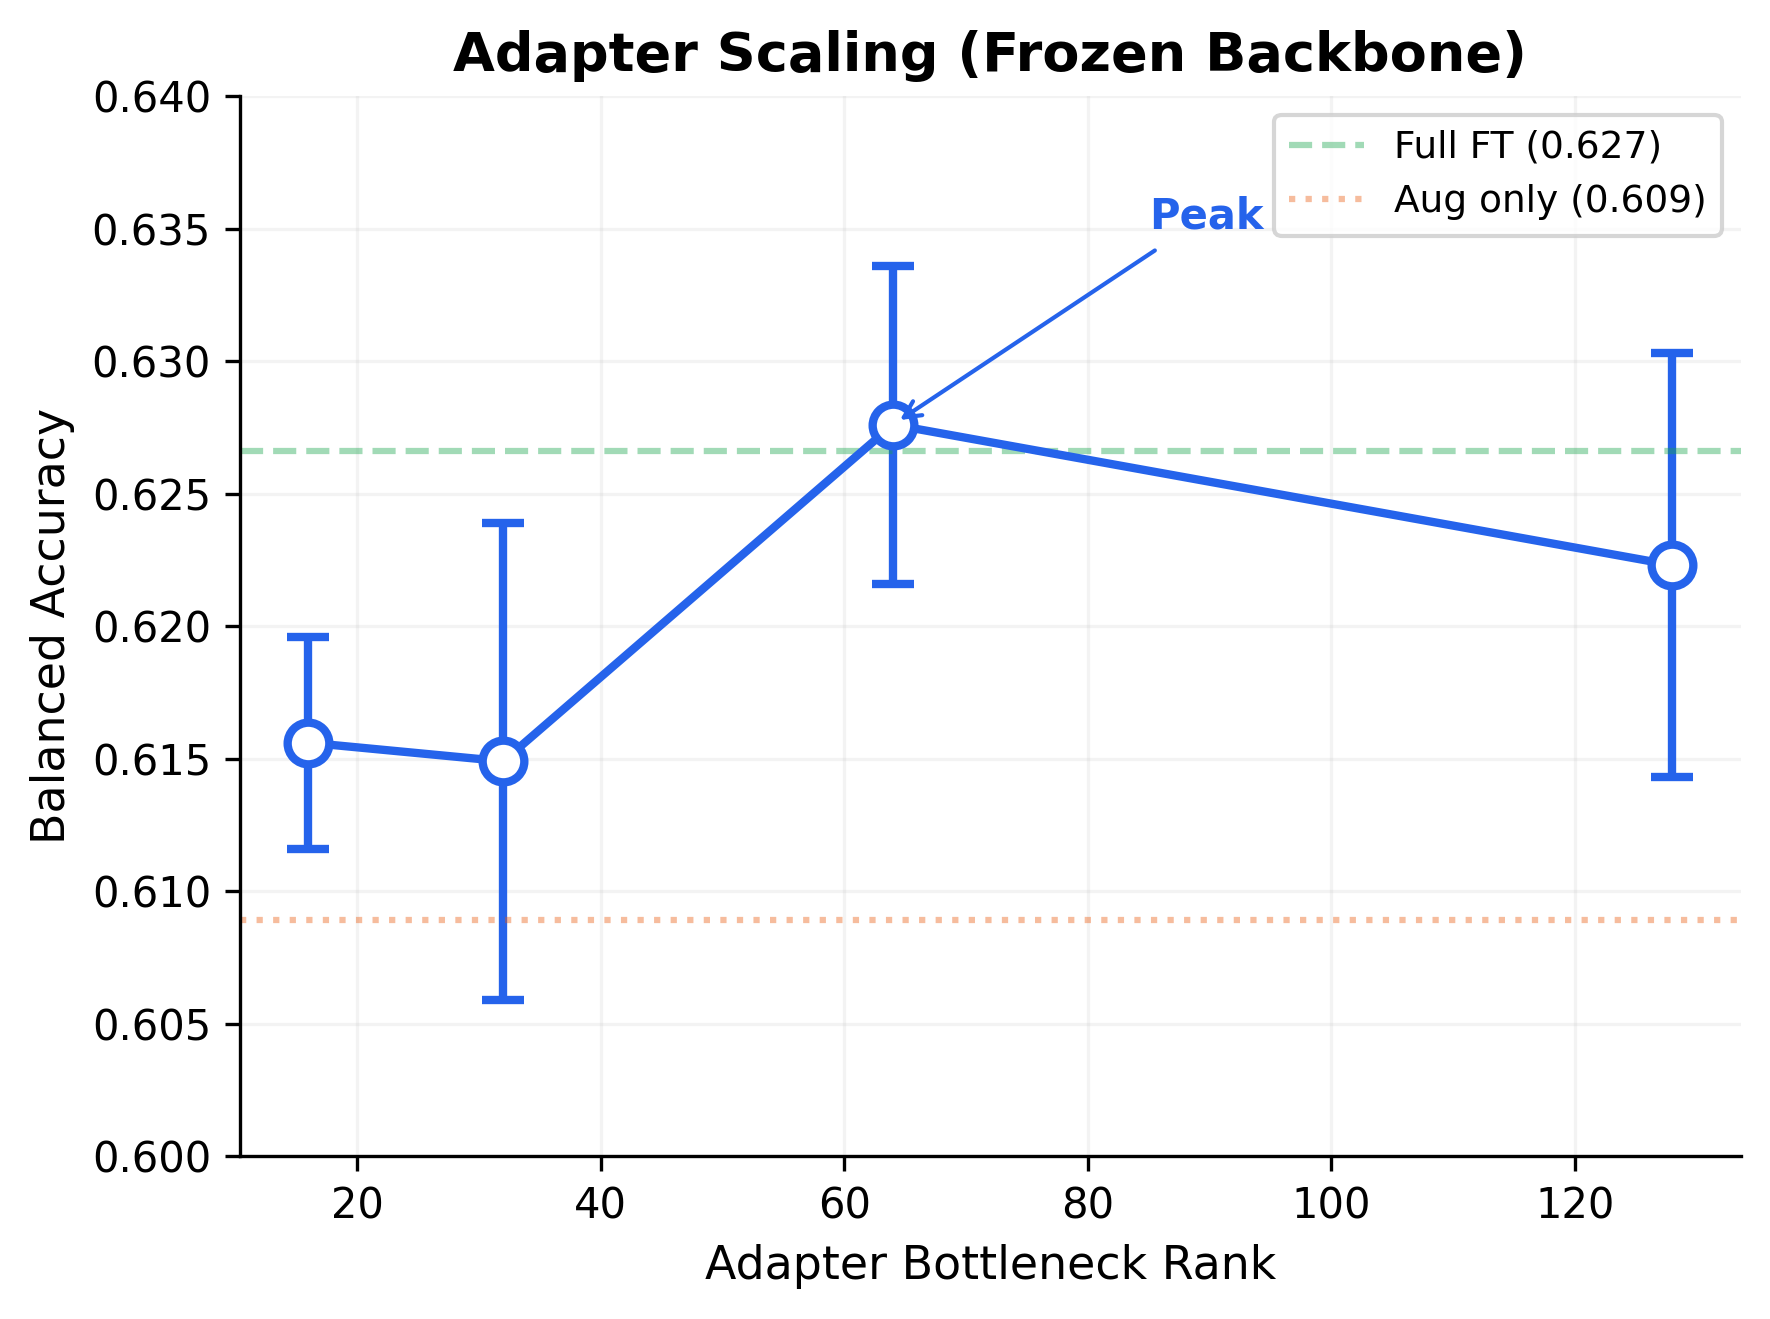
\includegraphics[width=\linewidth]{figs/adapter_scaling.png}
        \caption{Adapter scaling on FACED: peak at $r=64$.}
        \label{fig:adapter_scaling}
    \end{subfigure}
    \hfill
    \begin{subfigure}[b]{0.48\textwidth}
        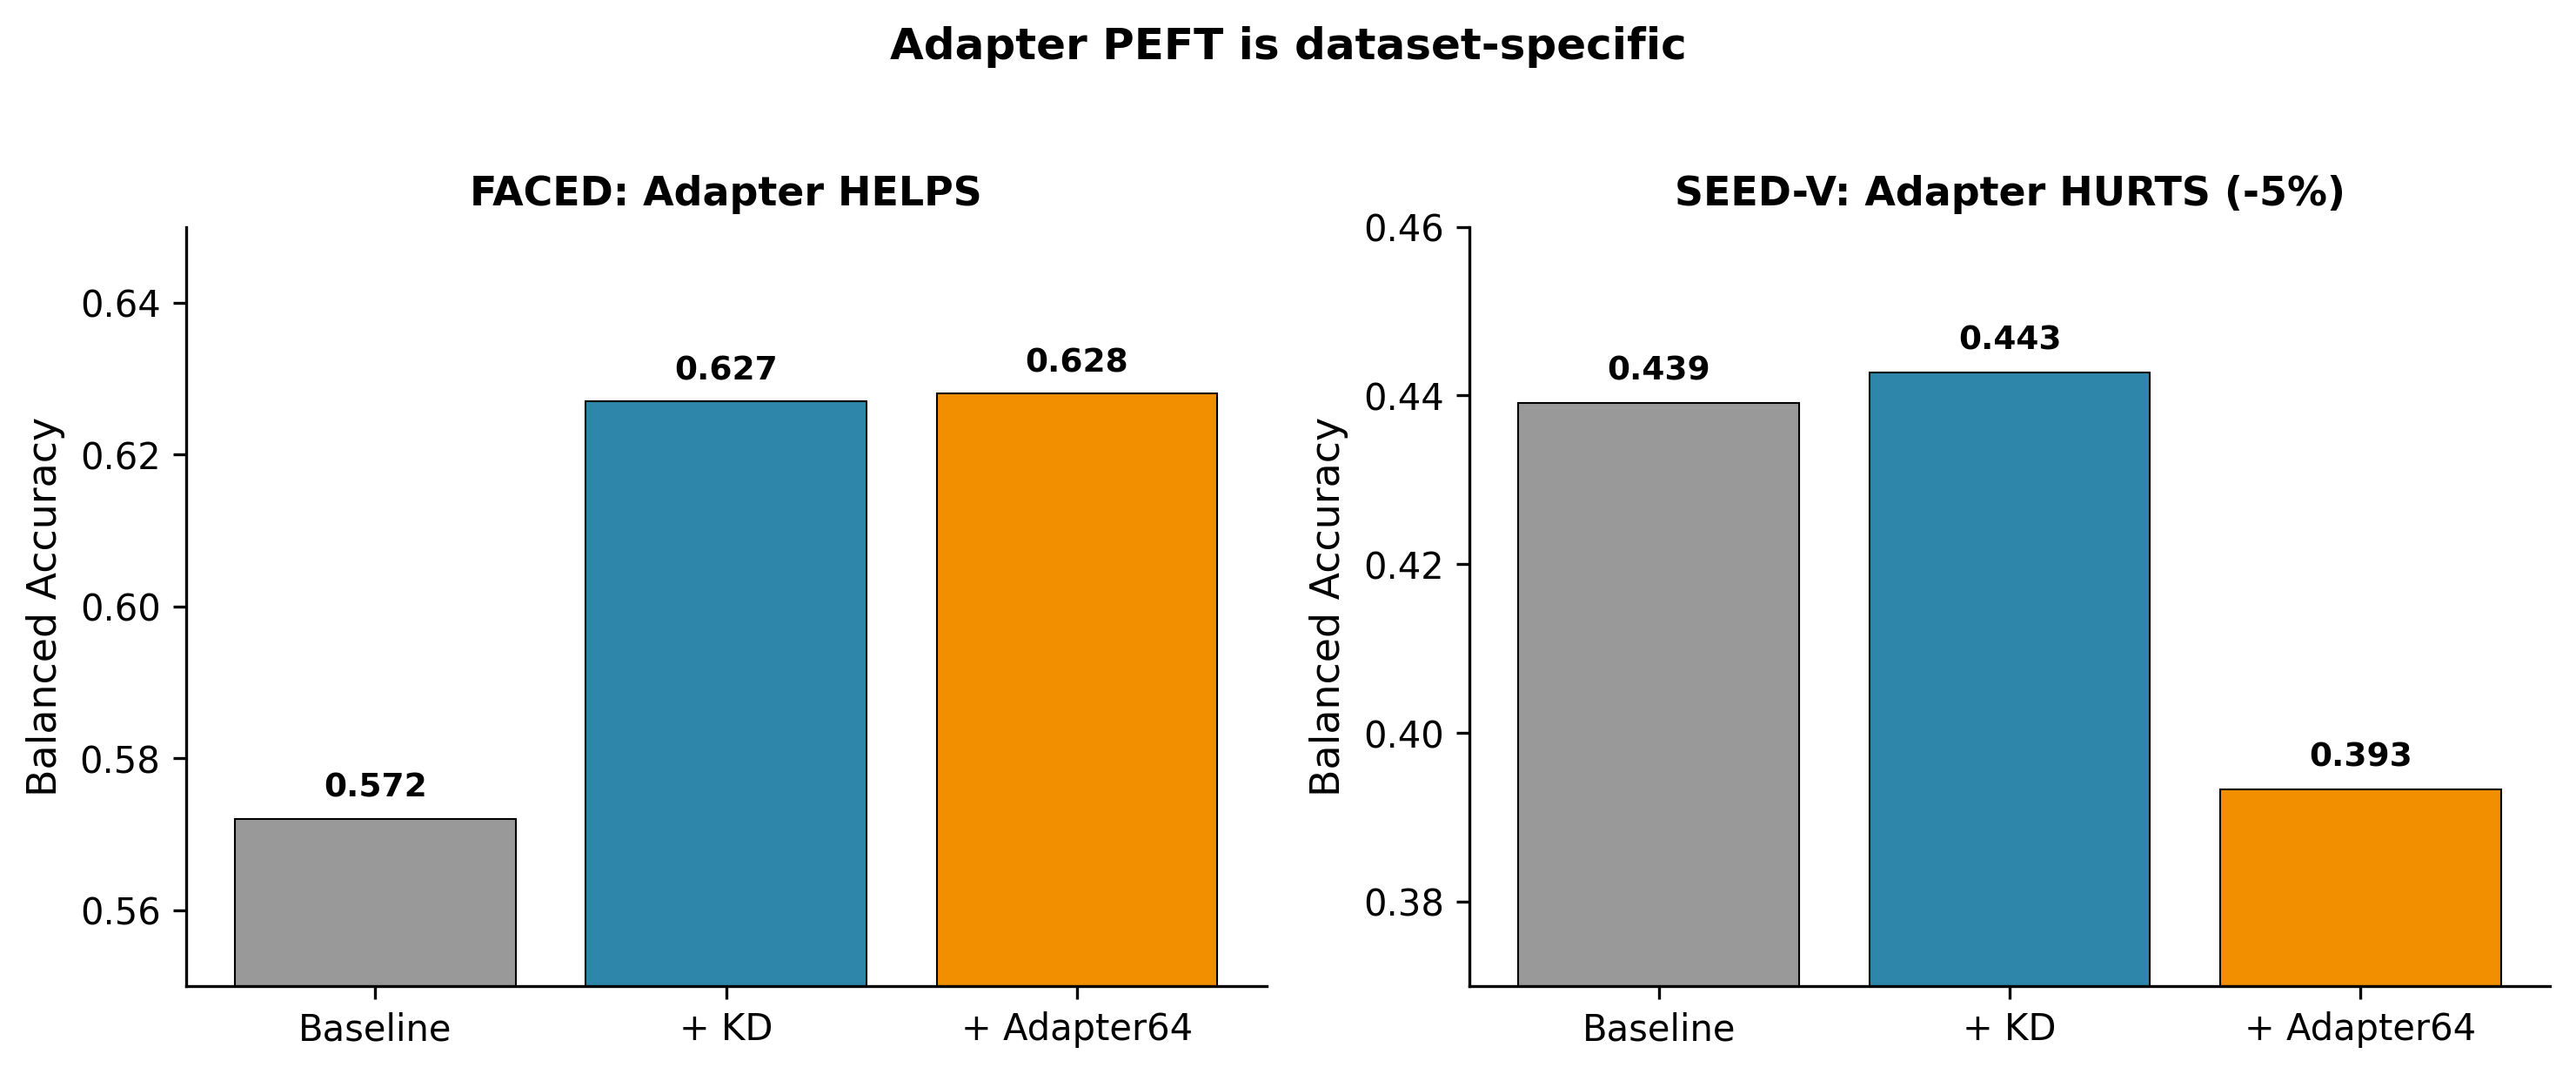
\includegraphics[width=\linewidth]{figs/fig_adapter_dataset_specific.png}
        \caption{Adapter PEFT helps FACED but hurts SEED-V.}
        \label{fig:adapter_ds}
    \end{subfigure}
    \caption{(a) Adapter bottleneck scaling on FACED. Performance peaks at $r = 64$ ($0.628$), then decreases for $r = 128$ ($0.622$) due to overfitting with frozen backbone. (b) The same PEFT recipe behaves \emph{oppositely} on the two datasets: $+9.8\%$ on FACED but $-5.0\%$ on SEED-V (CBraMod, 5\,s).}
    \label{fig:adapter_analysis}
\end{figure}

We systematically evaluate three PEFT approaches with frozen backbone: bottleneck adapters (rank 16/32/64/128), LoRA~\cite{hu2022lora} (rank 4/8/16), and FiLM conditioning~\cite{perez2018film} (3/6 modulation layers). The adapter scaling curve (\cref{fig:adapter_scaling}) shows a clear peak at $r=64$: $r=16$ ($0.616$) $\to$ $r=32$ ($0.615$) $\to$ $r=64$ ($\mathbf{0.628}$) $\to$ $r=128$ ($0.622$). LoRA achieves $\sim$$0.619$ across ranks (4/8/16), and FiLM ($0.612$--$0.615$) provides a complementary perspective but does not match adapter performance. Training adapters with frozen backbone ($0.628$) outperforms unfreezing the backbone after adapter warmup ($0.615$), demonstrating that CBraMod's pretrained representations benefit from being preserved intact.

\noindent\textbf{Negative finding: adapters do not transfer to SEED-V.} \cref{fig:adapter_ds} shows that the same adapter64 recipe that yields the FACED SOTA \emph{degrades} CBraMod by $5.0\%$ on SEED-V 5\,s ($0.443 \to 0.393$), and produces no benefit for LaBraM SEED-V either ($0.386$, indistinguishable from baseline $0.387$). This dataset-specific behavior is one of the more surprising findings of our study. We hypothesize two contributing factors: (i) SEED-V's smaller class set (5 emotions) and longer trial chunks place a greater premium on adapting the entire feature distribution, which a small bottleneck adapter cannot do; and (ii) the frozen pretrained features are well-aligned with FACED's 32-channel 10--20 layout but less so with SEED-V's 62-channel 10--10 layout, making the unfreeze-friendly full-FT pipeline more competitive on SEED-V. We report this negative result honestly: parameter-efficient fine-tuning is not a universal recipe across EEG datasets, and the choice between PEFT and full FT should be informed by both class structure and channel topology.

\subsection{Error Pattern and LLM Emotion Geometry}
\label{sec:analysis}
\vspace{-1mm}

\begin{figure}[!t]
    \centering
    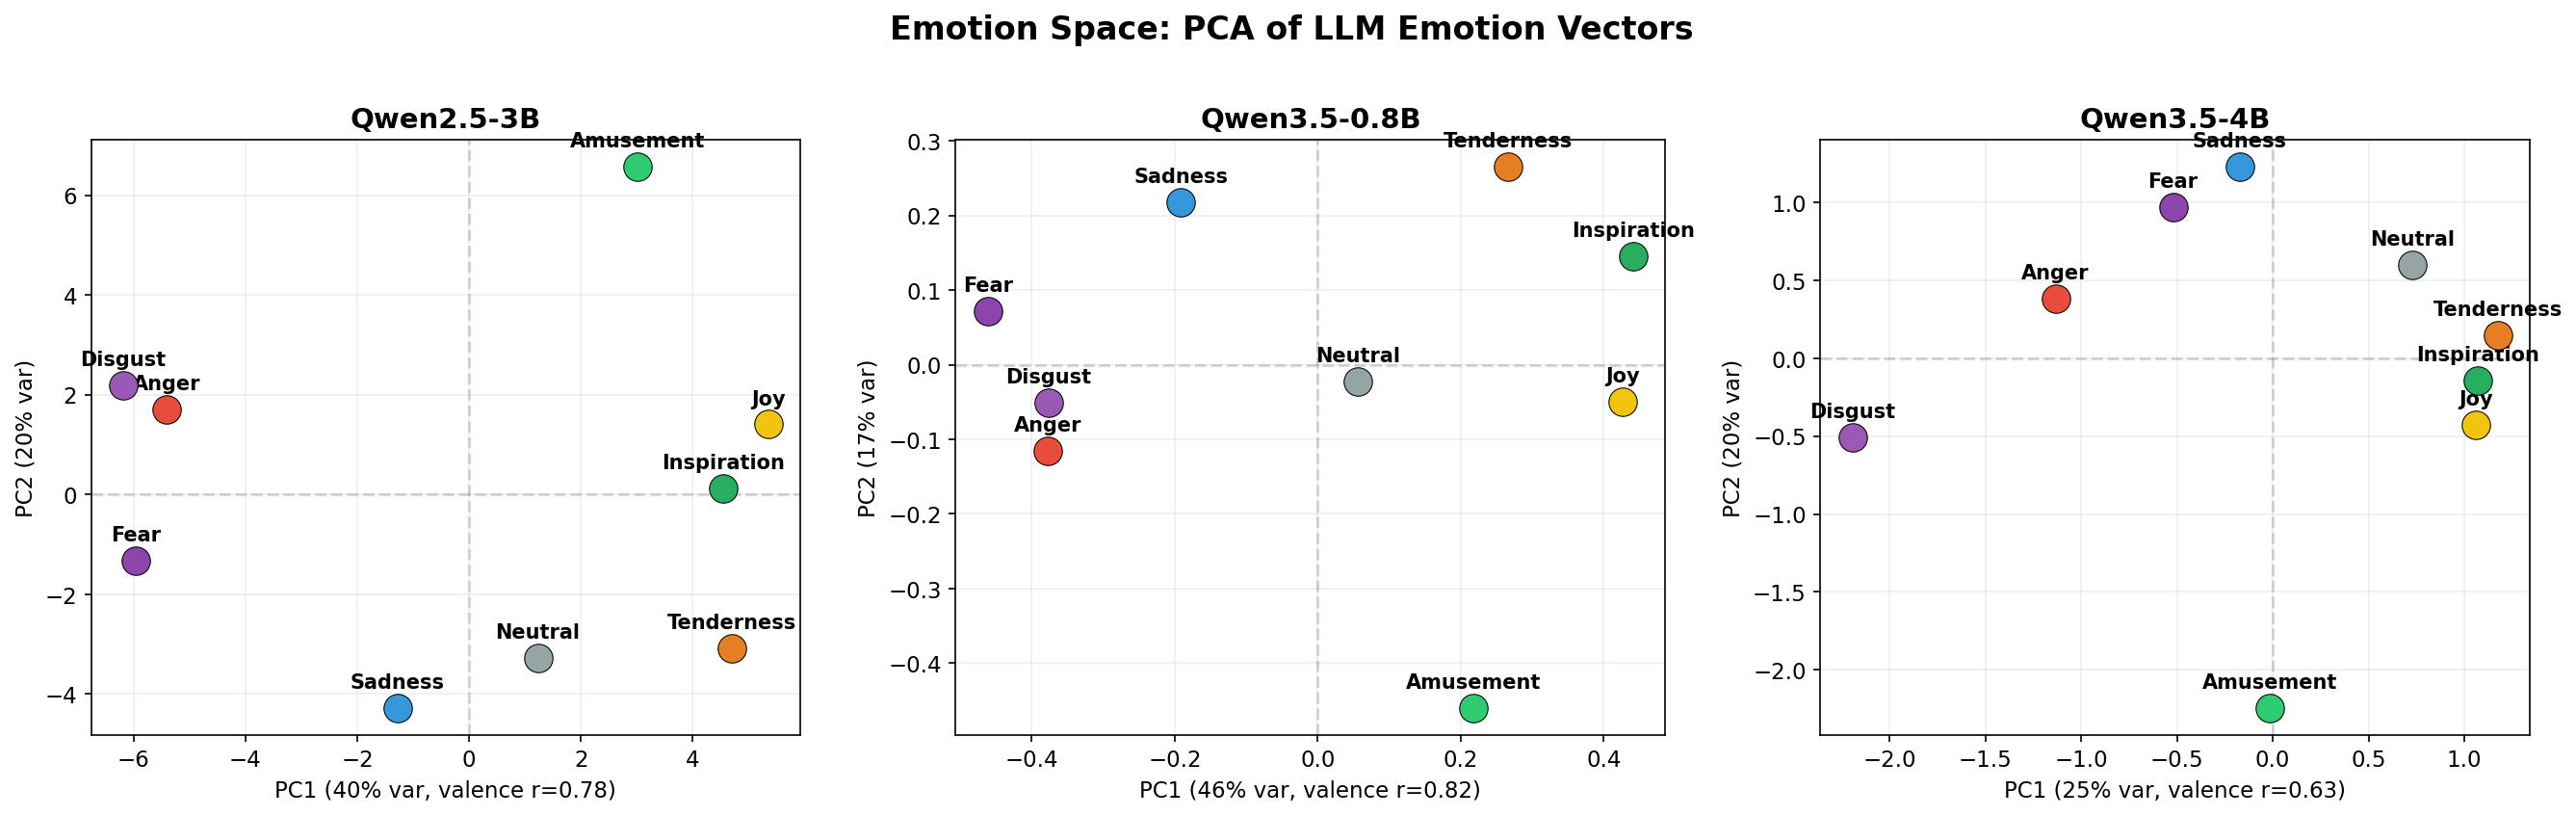
\includegraphics[width=\textwidth]{figs/fig1_pca_circumplex.png}
    \caption{PCA of Qwen2.5-0.5B emotion vectors recovers the full valence$\times$arousal circumplex~\cite{russell1980circumplex}. PC1 separates positive from negative valence; within the negative cluster, high-arousal emotions (anger, fear, disgust) separate from low-arousal sadness along PC2, mirroring the two-dimensional structure established in affective science.}
    \label{fig:pca}
\end{figure}

\begin{figure*}[!t]
    \centering
    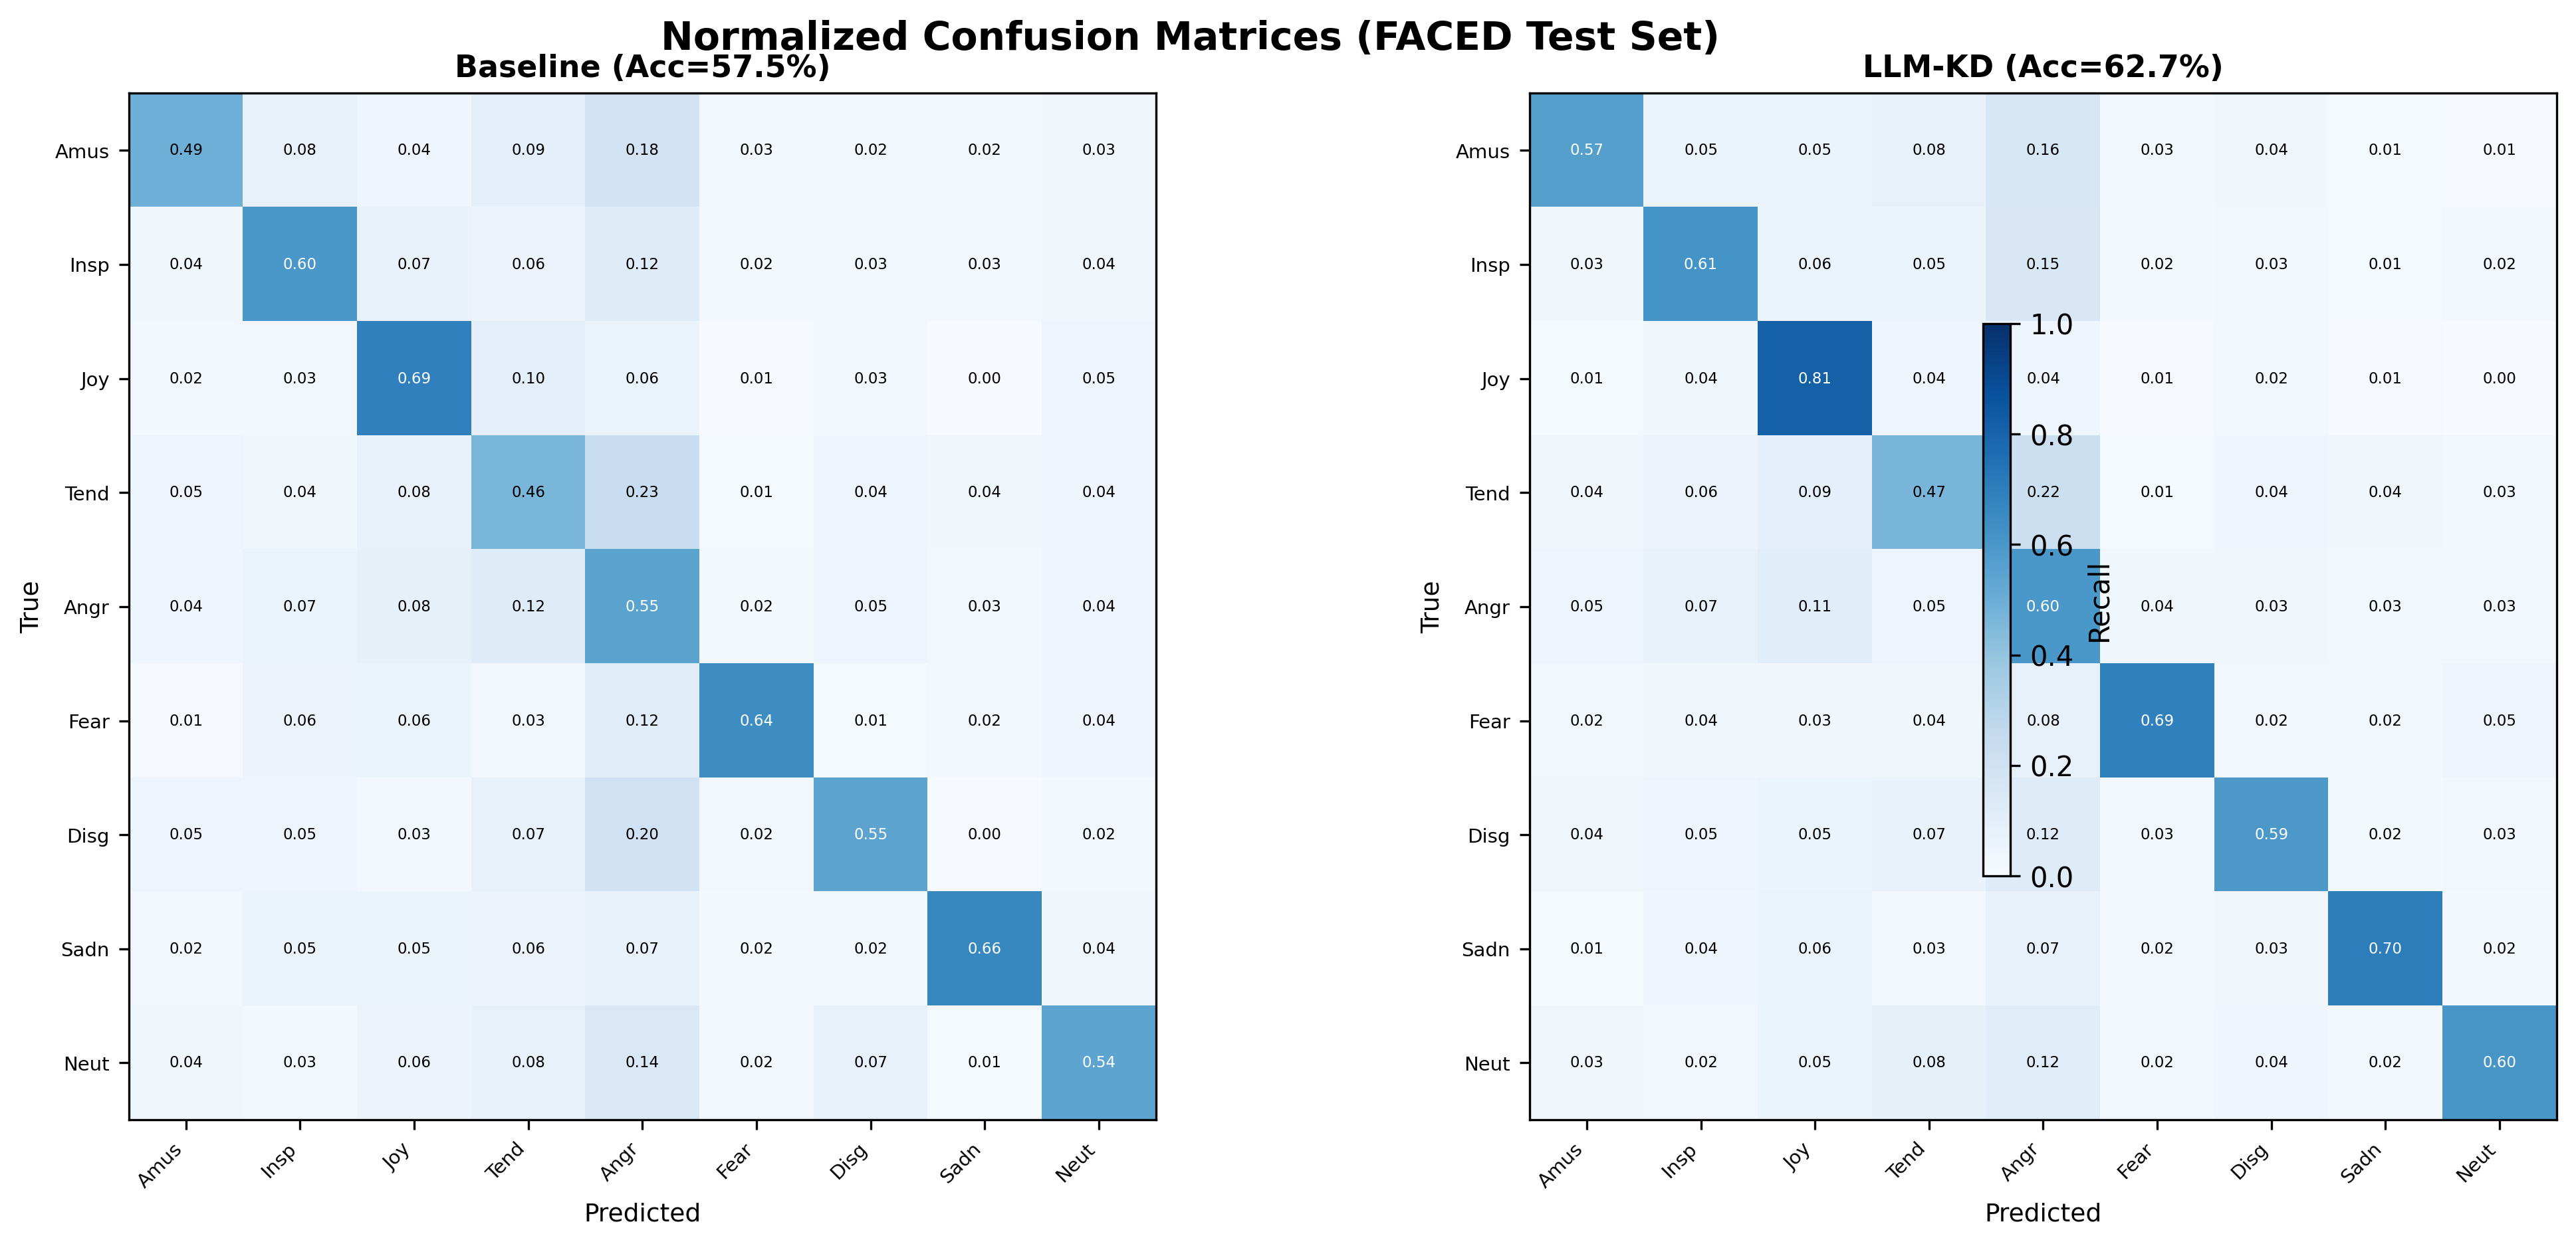
\includegraphics[width=\textwidth]{figs/confusion_matrices.png}
    \caption{Confusion matrices on FACED test set (seed 3407): CBraMod baseline (left, B.Acc $= 0.576$) vs.\ \ours KD (right, B.Acc $= 0.628$). Per-class recall improvements: Joy $+12.1\%$, Amusement $+7.2\%$, Neutral $+6.3\%$, Anger $+5.4\%$, Fear $+4.8\%$, Disgust $+4.8\%$, Sadness $+3.9\%$, Inspiration $+1.4\%$, Tenderness $+0.5\%$.}
    \label{fig:confusion}
\end{figure*}

\noindent\textbf{Error pattern.} EEG misclassification errors follow LLM semantic similarity (Spearman $r = 0.38$, $p = 3.4 \times 10^{-6}$). The effect is driven by negative-emotion confusions ($64.6\%$ of within-category errors, $p = 3.2 \times 10^{-13}$). Controls show that SBERT text descriptions ($r = 0.40$) are also strong predictors, while single-word embeddings and random vectors produce null results---indicating that the predictive structure lives in the LLM's full sentence-level representation, not in token-level word identities.

\noindent\textbf{Per-class improvement.} Confusion-matrix analysis (\cref{fig:confusion}) shows the largest gains on high-arousal positive emotions: joy ($+12.1\%$), amusement ($+7.2\%$), and on the high-arousal negative cluster: anger ($+5.4\%$), fear ($+4.8\%$), disgust ($+4.8\%$). Sadness, the only low-arousal negative emotion, shows a smaller gain ($+3.9\%$). This pattern is consistent with the LLM emotion geometry: the extracted vectors recover not just the valence axis but the full valence$\times$arousal circumplex, placing sadness apart from the high-arousal negative cluster. The KD loss exploits this two-dimensional structure, providing graded supervision that distinguishes both valence \emph{and} arousal.

\noindent\textbf{Per-subject analysis.} Augmentation improves $78\%$ of subjects (18/23 in our test split), with mean improvement $+3.8\%$ and maximum $+15.1\%$. Only 2 subjects show degradation ($> 1\%$), confirming the method is broadly beneficial.

\subsection{LLM Scale and Cross-Family Universality}
\label{sec:llm_scale}
\vspace{-1mm}

\begin{figure}[!t]
    \centering
    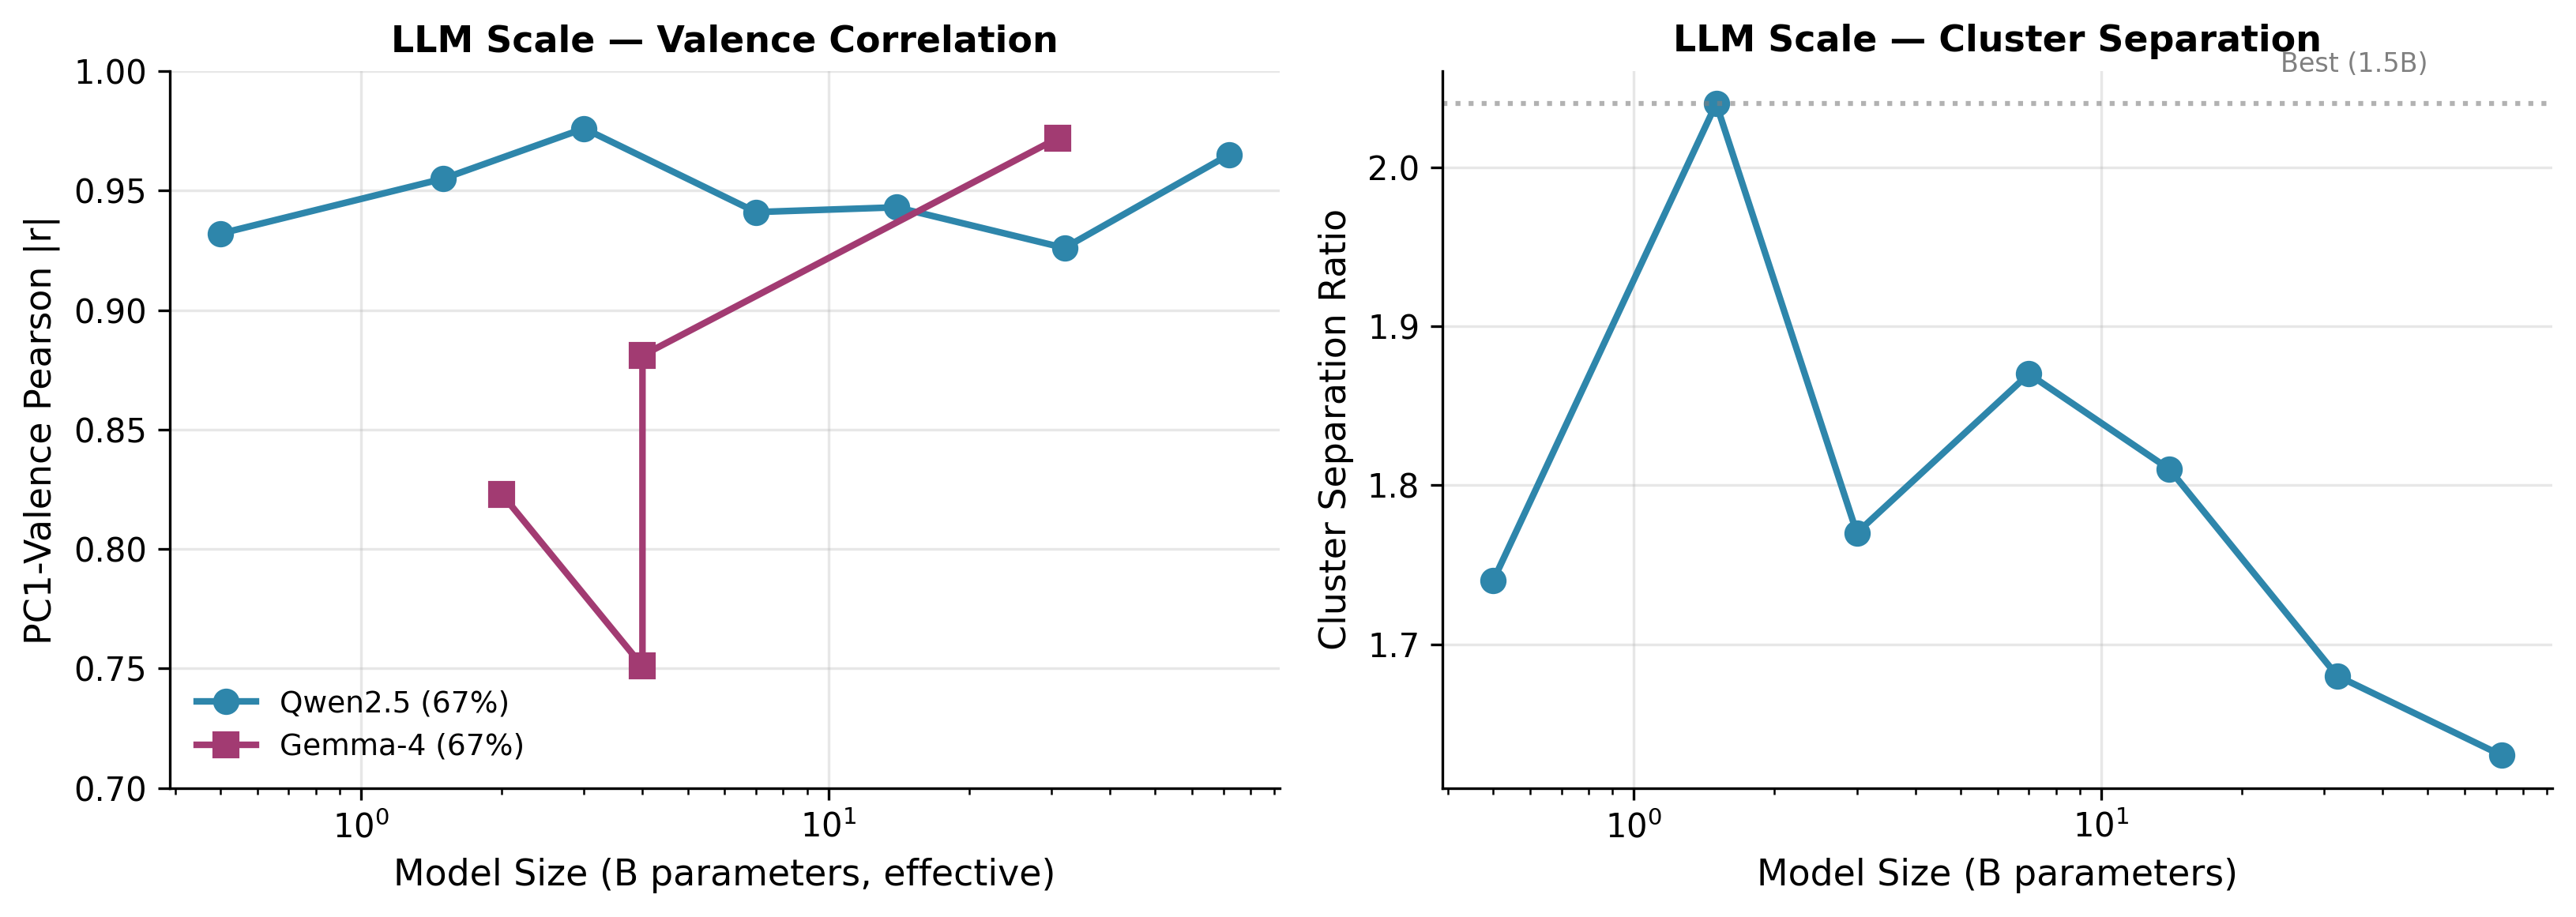
\includegraphics[width=0.96\linewidth]{figs/fig_llm_scale_dual.png}
    \caption{LLM scale analysis. \textbf{Left:} PC1--valence Pearson $|r|$ as a function of model size for Qwen2.5 and Gemma-4 families at the 67th-percentile layer. Qwen shows a U-shaped pattern (peak at 3B, dip at 32B, recovery at 72B). Gemma-4 shows a monotonic increase, peaking at 31B ($r = 0.972$). \textbf{Right:} Cluster separation ratio (inter-class vs intra-class distance) for Qwen sizes; this metric peaks at 1.5B ($2.04$) and declines monotonically with scale---the dimension that matters for KD soft-label informativeness.}
    \label{fig:llm_scale_dual}
\end{figure}

\begin{figure}[!t]
    \centering
    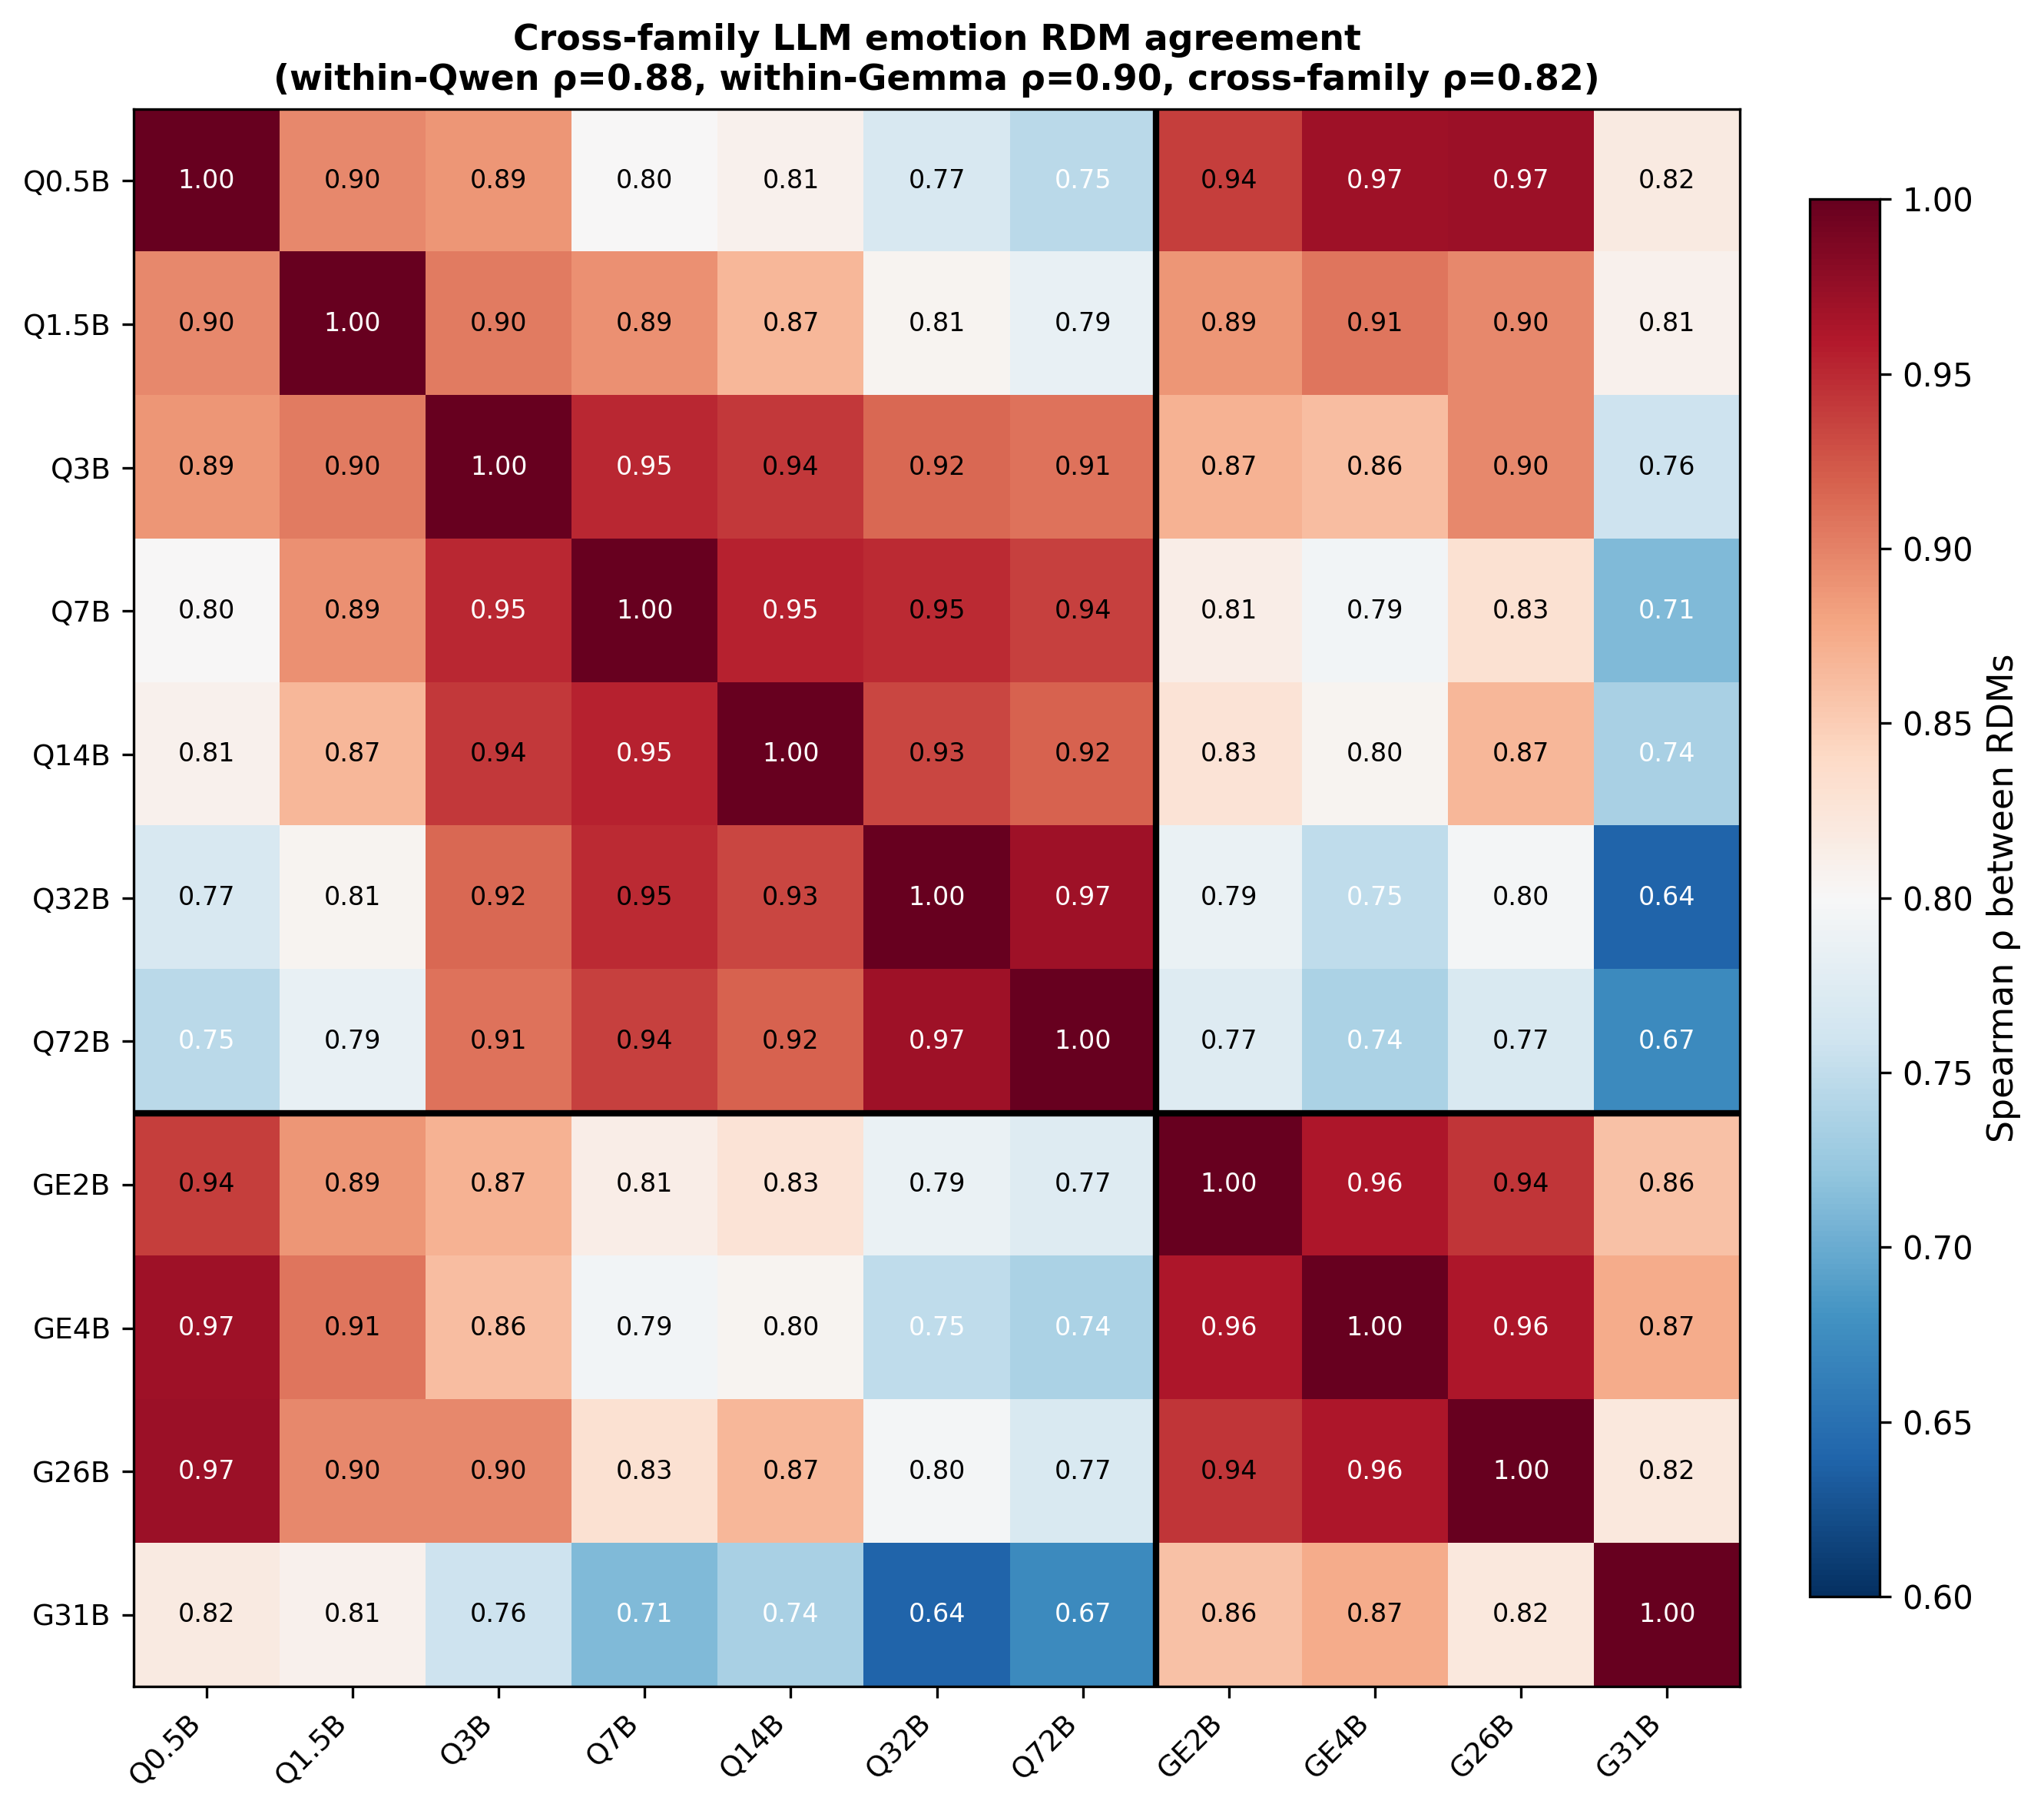
\includegraphics[width=0.85\linewidth]{figs/fig_cross_family_rdm.png}
    \caption{Cross-family RDM agreement matrix (Spearman $\rho$ between pairwise emotion-vector RDMs) for 11 instruction-tuned LLMs (7 Qwen sizes + 4 Gemma-4 variants). Within-family agreement (Qwen $\rho = 0.88$, Gemma $\rho = 0.90$) is only marginally higher than cross-family agreement ($\rho = 0.82$), confirming a universal LLM emotion geometry. Strongest cross-family pair: Qwen-0.5B $\leftrightarrow$ Gemma-4 26B-A4B at $\rho = 0.97$.}
    \label{fig:cross_family_rdm}
\end{figure}

We extend the LLM analysis to 11 instruction-tuned models from two families: 7 Qwen2.5 sizes (0.5B--72B) and 4 Gemma-4 variants (E2B, E4B, 26B-A4B, 31B). For each, we extract emotion vectors at both the 67th-percentile (default) and 29th-percentile (mid) layer, and analyze (i) PC1--valence Pearson correlation, (ii) cluster separation, and (iii) representational dissimilarity matrices.

\noindent\textbf{Scale dependence is metric-dependent.} \cref{fig:llm_scale_dual} reveals that ``which scale is best'' depends on the metric. For Qwen, valence correlation follows a U-shape (peak at 3B with $r = 0.976$, dip at 32B with $r = 0.926$, recovery at 72B with $r = 0.965$), while cluster separation peaks at 1.5B ($2.04$) and declines monotonically. The two metrics diverge because larger hidden dimensions ($896 \to 8192$) preserve the valence \emph{direction} (high $r$) while shrinking inter-class distances relative to the ambient space---the curse of dimensionality applied to emotion representations. For KD, cluster separation is the operationally relevant metric because it determines the informativeness of the soft labels. Thus Qwen-1.5B is the optimal teacher size, and---contra expectations---using the largest available LLM is not the right choice. Gemma-4 follows a different pattern: its 67\%-depth Pearson $r$ is monotonically increasing with size, peaking at $r = 0.972$ for the 31B dense model.

\noindent\textbf{Mid-layer extraction is family-dependent.} Drawing on prior interpretability work showing that emotion concepts concentrate in mid-layer self-attention~\cite{tak2025emotion_interpretability,decoding_emotion_deep2024}, we tested whether 29\%-depth extraction outperforms 67\%-depth. The result reverses with family. For Qwen, all 7 sizes show $r_{67\%} > r_{29\%}$ ($\sim$$0.94$ vs.\ $\sim$$0.83$ on average). For Gemma-4, the small models (E2B, E4B) show $r_{29\%} > r_{67\%}$ (mid-layer better), while the large models (26B-A4B, 31B) flip back to $r_{67\%} > r_{29\%}$, with Gemma-4 31B showing a striking gap ($0.972$ vs.\ $0.488$). The practical implication is that there is no universal ``use mid-layer'' rule; layer choice should be tuned per-family.

\noindent\textbf{Cross-family universality.} \cref{fig:cross_family_rdm} shows pairwise RSA between RDMs of all 11 models. Within-Qwen agreement averages $\rho = 0.883 \pm 0.067$, within-Gemma $\rho = 0.904 \pm 0.055$, and Qwen$\leftrightarrow$Gemma cross-family $\rho = 0.818 \pm 0.081$. The cross-family agreement is only $\sim$$7\%$ lower than within-family, providing strong empirical support for the claim that LLM emotion geometry is universal across instruction-tuned models. The strongest cross-family pair (Qwen-0.5B$\leftrightarrow$Gemma-4 26B-A4B at $\rho = 0.97$) involves models that differ in family, size, and architecture (dense vs MoE) yet share nearly identical emotion structure. We also confirmed via linear probing that all 11 models achieve $100\%$ binary cluster purity for positive vs negative emotions at appropriate depth, with perfect linear separability for Qwen-1.5B, Qwen-3B+, and Gemma-4 31B (\cref{sec:supp_llm}).

\noindent\textbf{SFT Negative Result.} We further investigated whether emotion-specific supervised fine-tuning (SFT) of the teacher LLM improves vector quality. Using LoRA instruction tuning with 189 emotion classification/explanation examples, cluster separation \emph{decreases} from $2.04$ (base) to $1.70$ ($-2.3\%$). Scaling to 1{,}898 instructions worsens the decline ($1.63$, $-6.3\%$), while the overall RDM geometry remains stable (RDM agreement $r = 0.992$). The emotion geometry present in instruction-tuned models thus emerges from broad language modeling; further emotion-specific tuning tightens categorical boundaries without enriching inter-class structure, producing less informative soft labels. This parallels findings in brain--LLM alignment, where scaling---but not instruction tuning beyond a threshold---increases representational correspondence~\cite{scaling_brain_alignment2024}.

\subsection{Representational Alignment via CKA}
\label{sec:cka}
\vspace{-1mm}

\begin{figure}[!t]
    \centering
    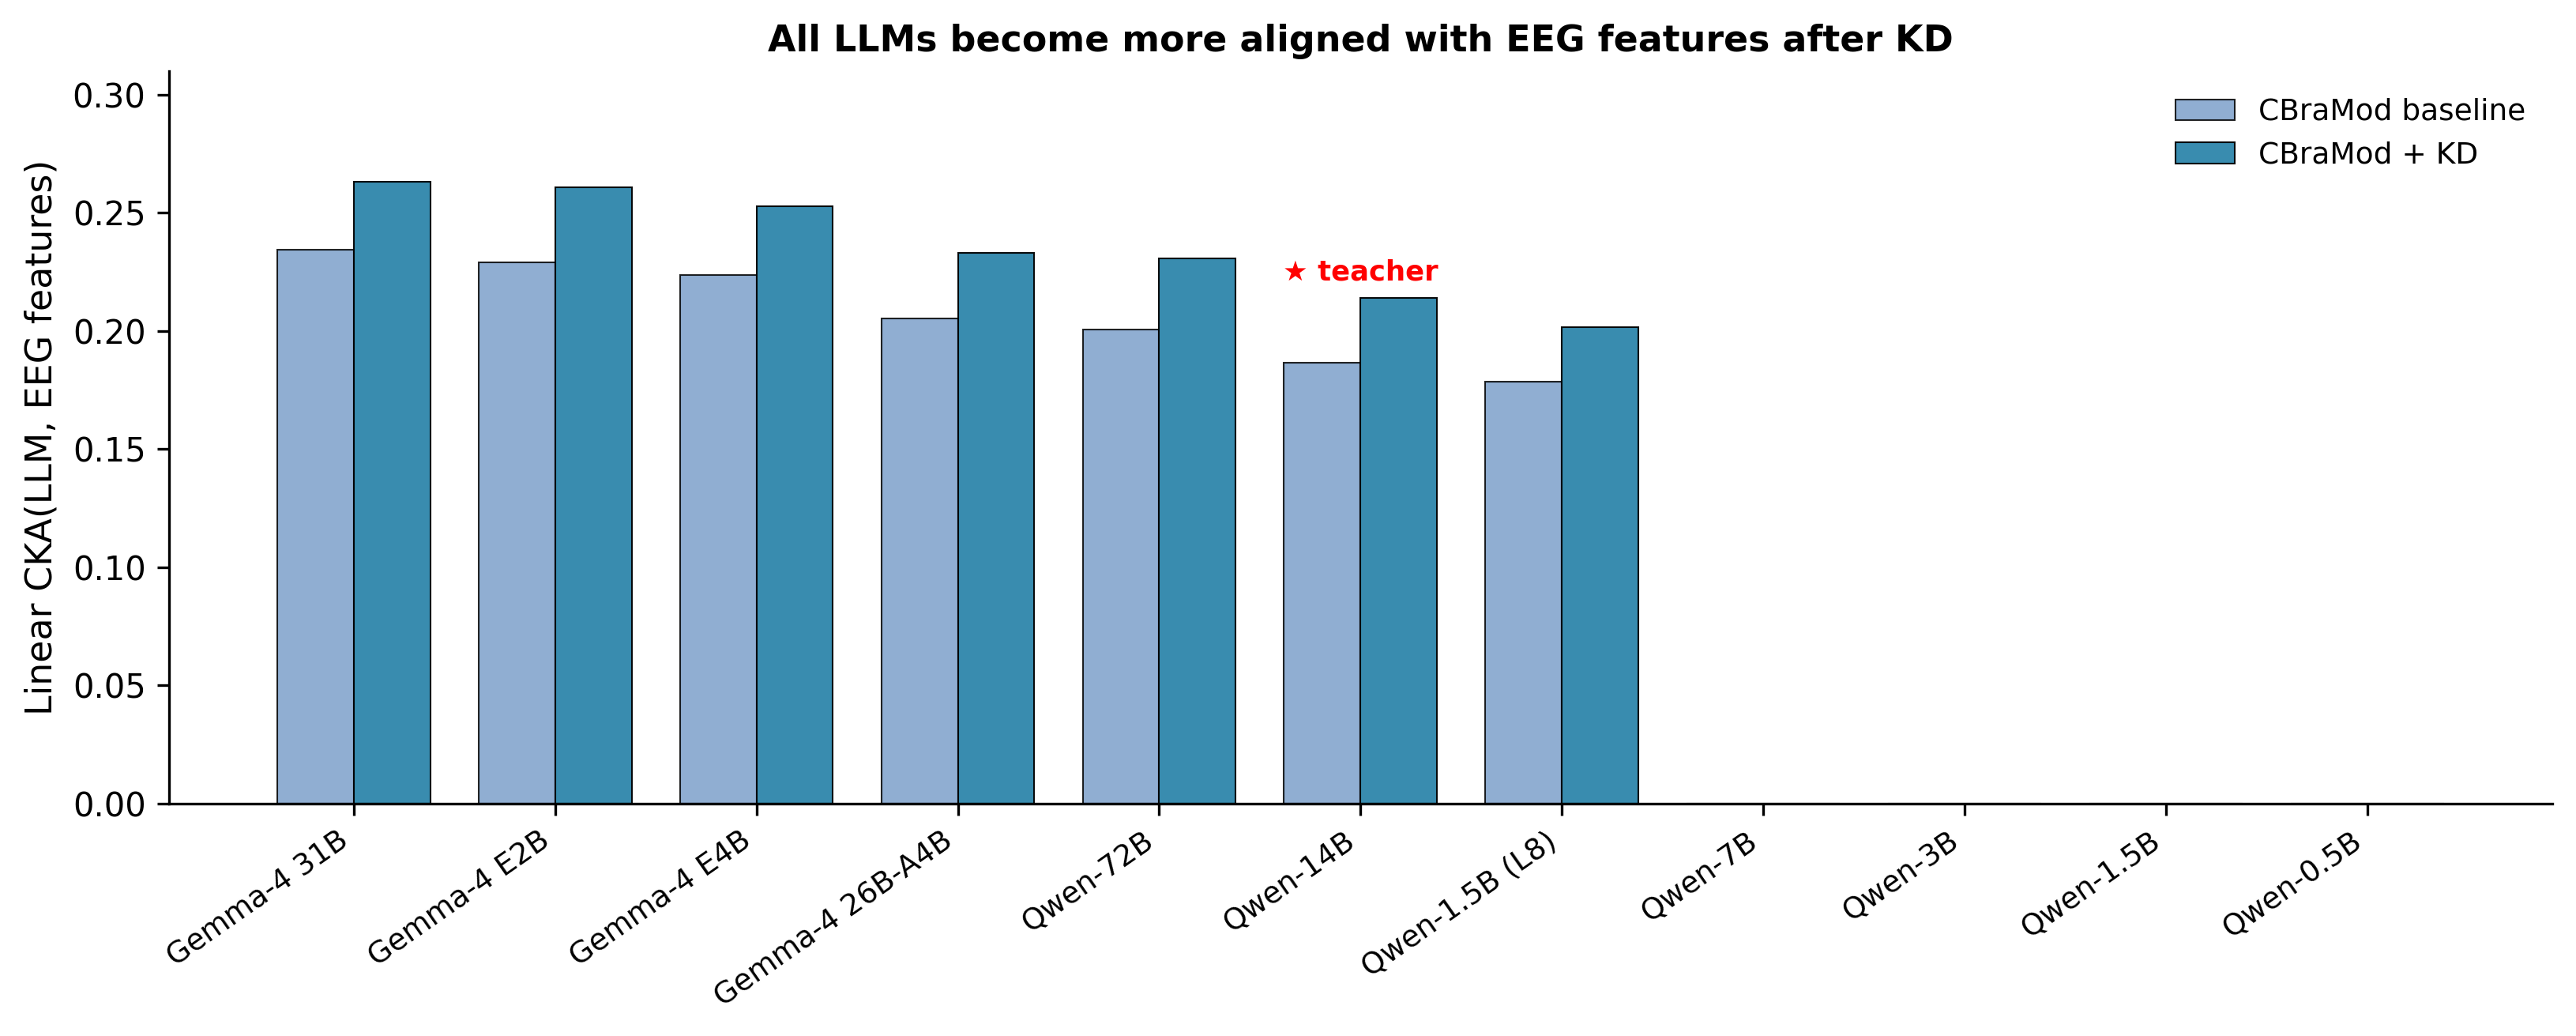
\includegraphics[width=0.96\linewidth]{figs/fig_cka_increase.png}
    \caption{Linear CKA between LLM per-sample features and CBraMod EEG penultimate features, baseline vs +KD. \emph{All 11 LLMs become more aligned with EEG features after KD} ($\Delta$CKA $\approx +0.03$ across the board). The teacher used for training (Qwen-14B, marked $\star$) is \emph{not} the most-aligned LLM after distillation: Gemma-4 31B has the highest CKA, indicating that KD absorbs a universal emotion structure rather than overfitting to one specific teacher.}
    \label{fig:cka_increase}
\end{figure}

To directly test whether KD makes the EEG model's representations more brain-LLM aligned---a claim that lies at the heart of our paper---we compute Linear Centered Kernel Alignment (CKA)~\cite{kornblith2019cka}, the standard metric for measuring representational similarity in NeurIPS-era brain-LLM alignment work~\cite{rethinking_cka_kd2024,brain_llm_compression2023}. For each test sample, we use the LLM emotion vector for that sample's class as a per-sample feature, and we compare these against CBraMod's penultimate features (200-dim) before and after KD on $1{,}932$ FACED test samples.

\cref{fig:cka_increase} shows a uniform pattern: \emph{every} LLM in our suite---including those from a different family from the training teacher---becomes \emph{more} CKA-aligned with CBraMod's features after KD, with $\Delta$CKA $\approx +0.03$ across the board (Linear CKA: $0.16 \to 0.19$ to $0.23 \to 0.26$ depending on the LLM). Notably, the highest post-KD alignment is achieved with Gemma-4 31B (CKA $= 0.263$), even though training used Qwen-14B as the teacher. This argues that KD does not simply pull EEG features toward the specific teacher; it absorbs a universal emotion structure that aligns with all sufficiently capable instruction-tuned LLMs. We find a similar pattern for kernel CKA (RBF) and for class-mean RSA, with Linear CKA showing the cleanest signal.

\subsection{Representational Visualization (t-SNE)}
\label{sec:tsne}
\vspace{-1mm}

\begin{figure*}[!t]
    \centering
    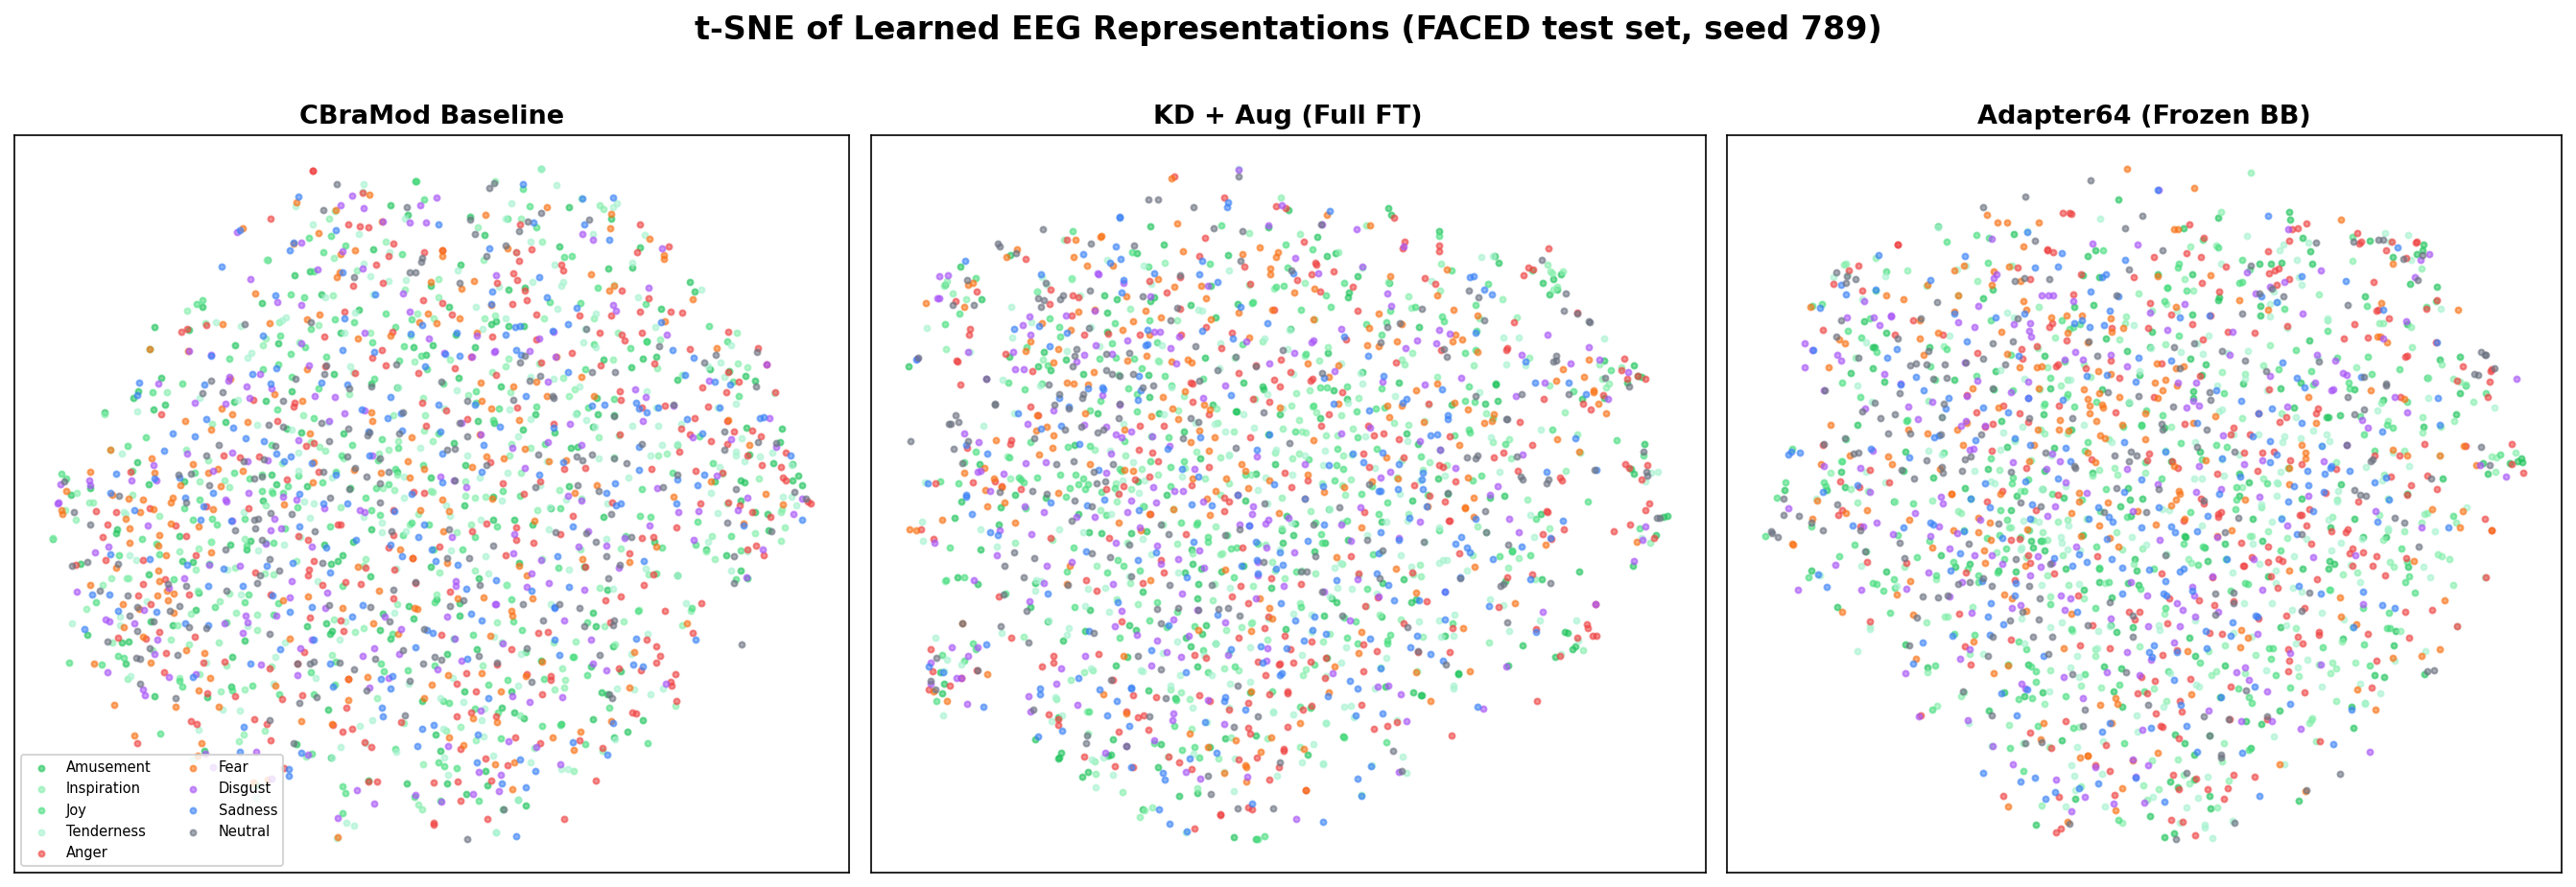
\includegraphics[width=\textwidth]{figs/fig_tsne_comparison.png}
    \caption{t-SNE visualization of learned EEG representations on the FACED test set. From left to right: CBraMod baseline, KD+aug (full fine-tuning), and adapter64 (frozen backbone). Emotion clusters become progressively more distinct with each component of \ours.}
    \label{fig:tsne}
\end{figure*}

\begin{figure}[!t]
    \centering
    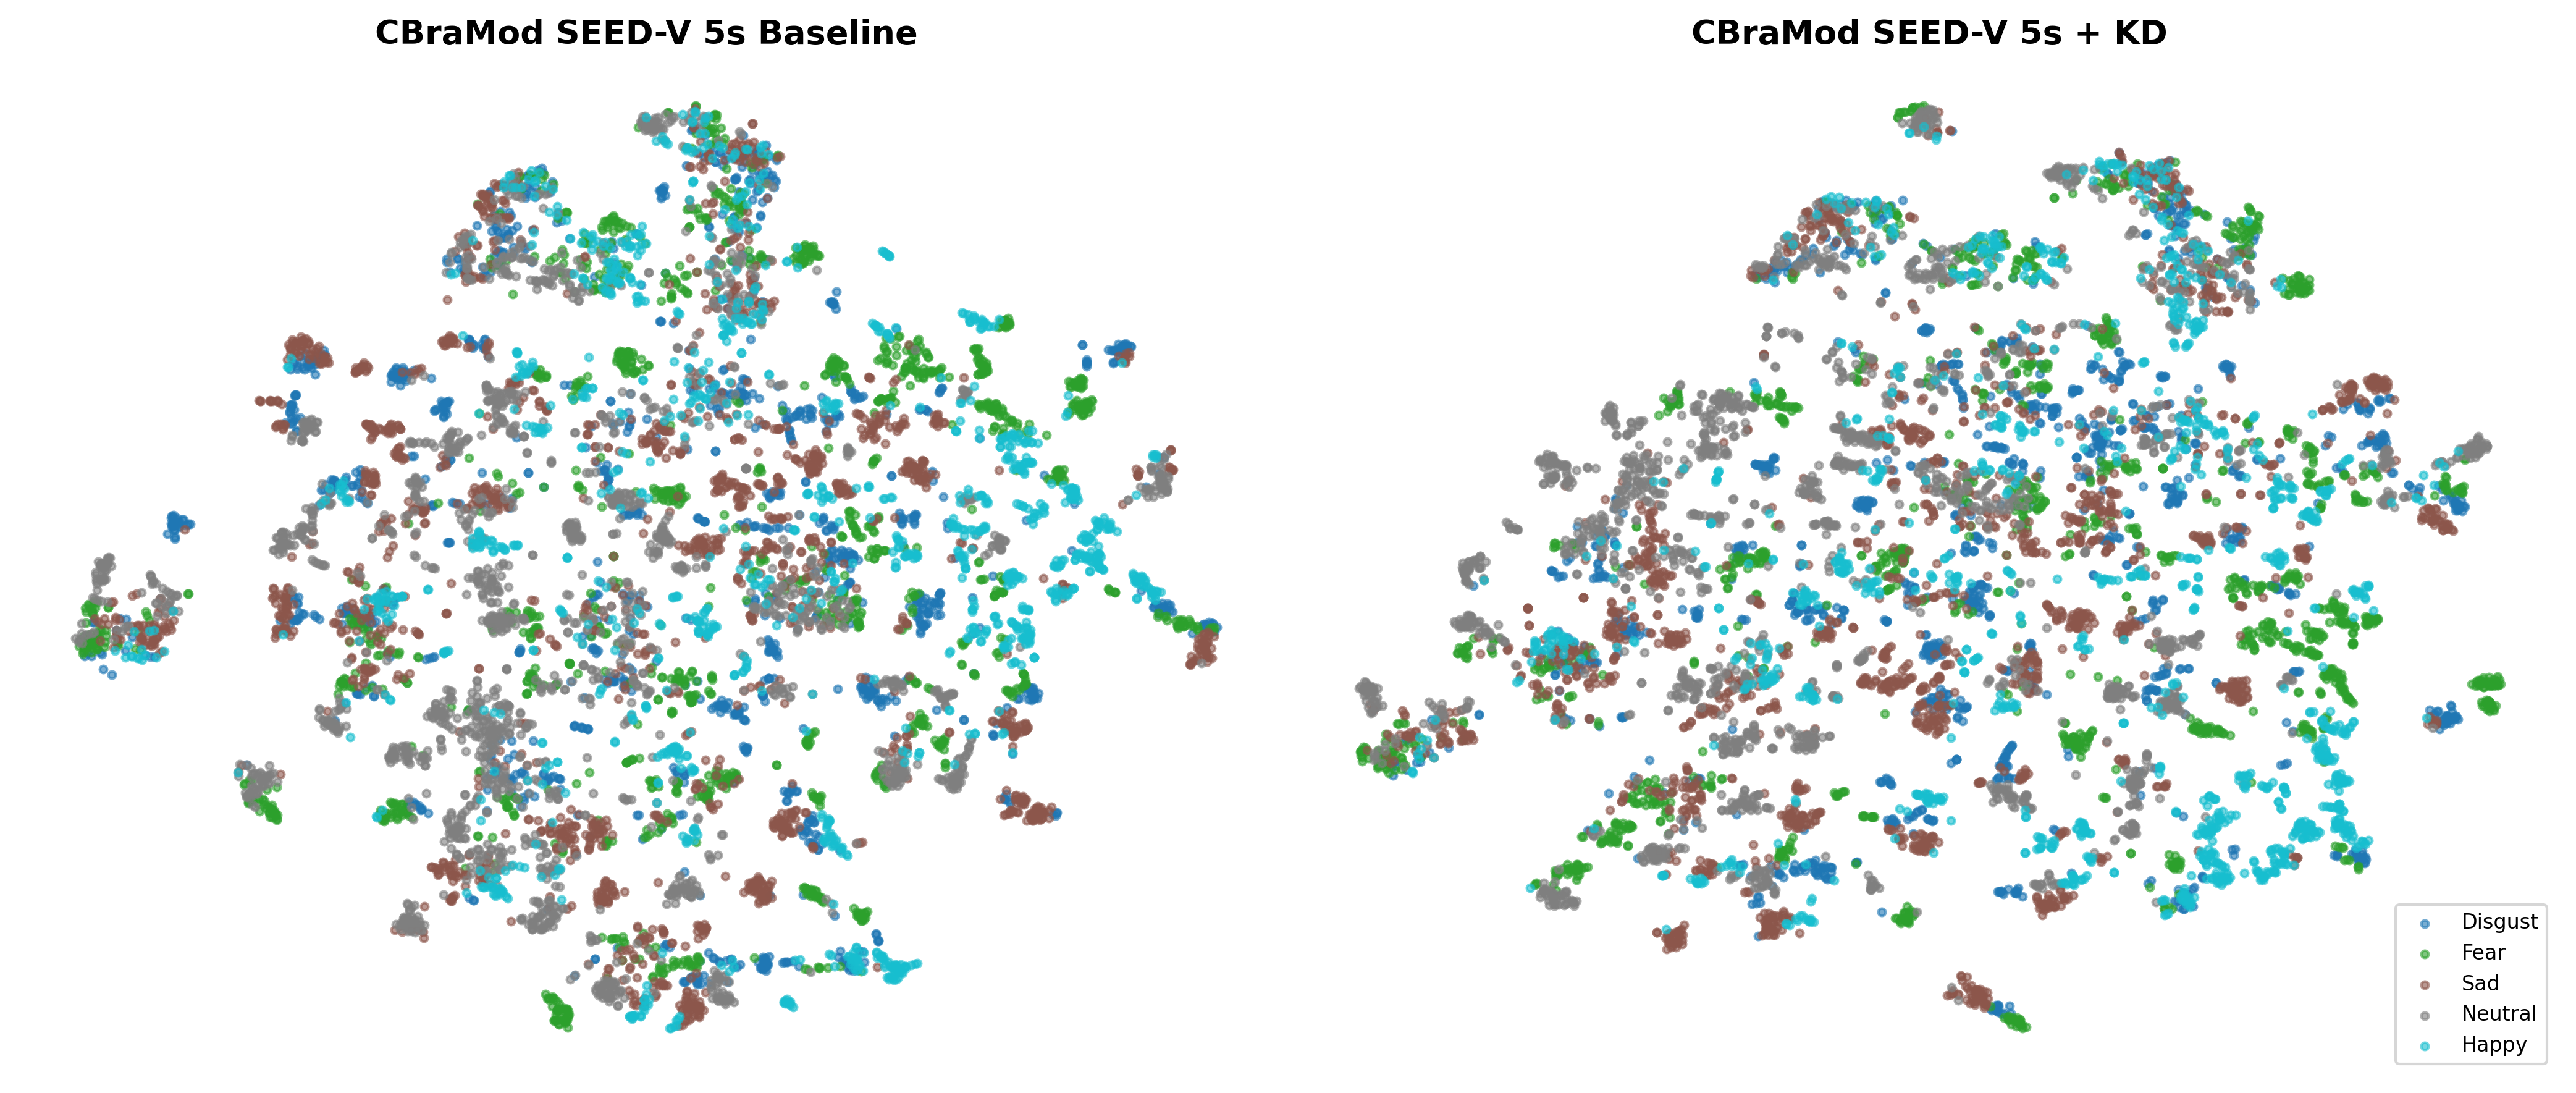
\includegraphics[width=0.95\linewidth]{figs/fig_seedv_tsne.png}
    \caption{t-SNE of CBraMod SEED-V 5\,s features, baseline vs.\ +KD (seed 3407). KD increases inter-class separation for high-arousal emotions (Fear $+4.4\%$, Disgust $+2.7\%$, Happy $+3.1\%$), with a small decrease for Sad ($-4.4\%$). The improvement is much smaller than on FACED, consistent with the lower headroom and the partial KD effect ($+0.83\%$, CI excludes zero).}
    \label{fig:tsne_seedv}
\end{figure}

\cref{fig:tsne} shows t-SNE projections of CBraMod features on FACED across the baseline, +KD, and +Adapter64 stages of \ours. Emotion clusters become progressively more discrete with each component. \cref{fig:tsne_seedv} shows the analogous comparison for SEED-V 5\,s, where the smaller KD effect is reflected in subtler separation changes that nonetheless concentrate on the high-arousal classes most consistent with the LLM-driven supervision.

\subsection{Statistical Robustness via Bootstrap CIs}
\label{sec:bootstrap}
\vspace{-1mm}

\begin{table}[!t]
\caption{Bootstrap 95\% confidence intervals (10{,}000 resamples) for the main paired comparisons in this paper. CIs that exclude zero indicate effects that are reliable beyond the assumptions of paired $t$-tests. All comparisons are paired across 5 seeds.}
\small
\centering
\begin{tabular}{lcccc}
\toprule
Comparison & $\Delta$ mean & 95\% CI & $t$ & $p$ \\
\midrule
\rowcolor{blond}
\textbf{CBraMod FACED KD vs Baseline} & $\mathbf{+0.052}$ & $[+0.046, +0.057]$ & $15.5$ & $\mathbf{1{\times}10^{-4}}$ \\
\rowcolor{blond}
\textbf{LaBraM FACED KD vs Baseline} & $\mathbf{+0.026}$ & $[+0.011, +0.037]$ & $3.5$ & $\mathbf{0.025}$ \\
CBraMod SEED-V 5\,s KD vs Base & $+0.0036$ & $[+0.0001, +0.0074]$ & $1.8$ & $0.15$ \\
LaBraM SEED-V 19ch$\times$5\,s KD vs Base & $+0.018$ & $[+0.008, +0.028]$ & $3.1$ & $\mathbf{0.037}$ \\
Qwen-1.5B vs 0.5B (mid-layer KD) & $+0.015$ & $[+0.006, +0.024]$ & $2.8$ & $\mathbf{0.047}$ \\
Best teacher (1.5B L8) vs 0.5B 67\% & $+0.004$ & $[-0.001, +0.009]$ & $1.3$ & $0.25$ \\
\bottomrule
\end{tabular}
\label{tab:bootstrap}
\end{table}

\cref{tab:bootstrap} reports bootstrap 95\% percentile confidence intervals for all key comparisons in this paper. Bootstrap CIs are robust to non-normality of the seed-level differences and complement our paired $t$-tests. The two headline cross-backbone results (CBraMod FACED, LaBraM FACED) have CIs that are far from zero. The cross-dataset SEED-V results show CIs that exclude zero even when paired $t$-tests are marginal (CBraMod 5\,s) or significant (LaBraM 19ch$\times$5\,s). The ``best teacher'' comparison (Qwen-1.5B layer 8 vs.\ Qwen-0.5B 67\%) shows a CI that crosses zero ($[-0.001, +0.009]$): the two teachers are empirically indistinguishable at $n = 5$, so we keep the simpler 0.5B--67\% configuration as our paper SOTA.

\subsection{Computational Efficiency}
\label{sec:efficiency}
\vspace{-1mm}

\begin{wraptable}[14]{r}{0.5\textwidth}
\centering
\vspace{-5mm}
\caption{Parameter and inference cost breakdown. CBraMod's classifier head dominates total parameters; the pretrained backbone is only 4.88M. KD adds a small training-only semantic head with zero inference cost; adapter64 adds 310K trainable params and freezes the 4.88M backbone.}
\small
\begin{tabular}{lccc}
\toprule
Method & Total & Train & Backbone \\
\midrule
Baseline & 133.3M & 133.3M & 4.88M \\
+KD & 134.1M & 134.1M & 4.88M \\
+Adapter64 & 134.4M & 129.5M & frozen \\
\bottomrule
\end{tabular}
\label{tab:efficiency}
\end{wraptable}

We report a breakdown of \ours's parameter footprint in \cref{tab:efficiency}. CBraMod's backbone is only 4.88M parameters (matching the published spec~\cite{wang2025cbramod}), but the classifier head---a flatten + MLP that operates on $32 \times 10 \times 200 = 64{,}000$-dimensional inputs---is $128.4$M, dominating the total. KD adds a small training-only semantic projection head ($+0.83$M), and inference cost is identical to baseline because the semantic head is dropped at test time. Adapter64 adds $0.31$M adapter parameters and freezes the 4.88M backbone, preserving its pretrained features. The narrative for adapter PEFT in this setting is therefore not raw parameter savings (the classifier still dominates) but rather \emph{feature preservation}: the frozen backbone retains its TUEG-pretrained representations intact while the adapters provide task-specific residual paths.
